%%%%%%%%%%%%%%%%%%%% author.tex %%%%%%%%%%%%%%%%%%%%%%%%%%%%%%%%%%%
%
% sample root file for your "contribution" to a contributed volume
%
% Use this file as a template for your own input.
%
%%%%%%%%%%%%%%%% Springer %%%%%%%%%%%%%%%%%%%%%%%%%%%%%%%%%%


% RECOMMENDED %%%%%%%%%%%%%%%%%%%%%%%%%%%%%%%%%%%%%%%%%%%%%%%%%%%
\documentclass[graybox]{svmult}

% choose options for [] as required from the list
% in the Reference Guide

\usepackage{mathptmx}       % selects Times Roman as basic font
\usepackage{helvet}         % selects Helvetica as sans-serif font
\usepackage{courier}        % selects Courier as typewriter font
\usepackage{type1cm}        % activate if the above 3 fonts are
                            % not available on your system
%
\usepackage{makeidx}         % allows index generation
\usepackage{graphicx}        % standard LaTeX graphics tool
                             % when including figure files
\usepackage{epstopdf}

\usepackage[hang, small,labelfont=bf,up,textfont=it,up]{caption} % Custom captions under/above floats in tables or figures
\usepackage{subcaption}
\captionsetup{compatibility=false} % otherwise it raises some issues regarding compatibility

\usepackage{multicol}        % used for the two-column index
\usepackage[bottom]{footmisc}% places footnotes at page bottom
\usepackage{amsmath}
\usepackage{amssymb}
\usepackage{mathtools}
%\usepackage[linesnumbered, ruled, vlined]{algorithm2e}
%\usepackage{algorithm}% http://ctan.org/pkg/algorithms
%\usepackage{algorithmicx} 
%\usepackage{algpseudocode}% http://ctan.org/pkg/algorithmicx
%\renewcommand{\algorithmicrequire}{\textbf{Input:}}
%\renewcommand{\algorithmicensure}{\textbf{Output:}}
\usepackage{enumerate}
\usepackage{multirow}
\usepackage{cleveref}

\newcommand{\edit}[1]{{\color{black} #1}}

\usepackage{tikz}
\usepackage{pgfplots}
\usepackage{pgfplotstable}
\pgfplotsset{
    % most recent feature set of pgfplots
    compat=newest,
    % some settings for grid
    grid style={black!20!white, thin, densely dotted},
    % modify plot appearance
    every axis plot/.append style={no markers, thick},
    % i like the labels a bit smaller
    label style={font=\small},
    tick label style={font=\small}
}
\usepgfplotslibrary{external} 
\tikzexternalize[prefix=TikzFigures/]

%\usepackage[hang, small,labelfont=bf,up,textfont=it,up]{caption} % Custom captions under/above floats in tables or figures
\usepackage{booktabs} % Horizontal rules in tables
\usepackage{float} % Required for tables and figures in the multi-column environment - they need to be placed in specific locations with the [H] (e.g. \begin{table}[H])
%\usepackage{hyperref} % For hyperlinks in the PDF

% see the list of further useful packages
% in the Reference Guide

\makeindex             % used for the subject index
                       % please use the style svind.ist with
                       % your makeindex program

\pgfplotsset{every tick label/.append style={font=\Large}}

%%%%%%%%%%%%%%%%%%%%%%%%%%%%%%%%%%%%%%%%%%%%%%%%%%%%%%%%%%%%%%%%%%%%%%%%%%%%%%%%%%%%%%%%%

\begin{document}

\title*{Conservative Model Order Reduction for Fluid Flow}
% Use \titlerunning{Short Title} for an abbreviated version of
% your contribution title if the original one is too long
\author{Babak Maboudi Afkham, Nicol\`o Ripamonti, Qian Wang, and Jan S. Hesthaven}
% Use \authorrunning{Short Title} for an abbreviated version of
% your contribution title if the original one is too long
\institute{B. Maboudi Afkham, N. Ripamonti, Q. Wang, J.S. Hesthaven \at EPFL, Lausanne, Switzerland \email{babak.maboudi@epfl.ch}}
%
% Use the package "url.sty" to avoid
% problems with special characters
% used in your e-mail or web address
%
\maketitle

%\abstract*{Each chapter should be preceded by an abstract (10--15 lines long) that summarizes the content. The abstract will appear \textit{online} at \url{www.SpringerLink.com} and be available with unrestricted access. This allows unregistered users to read the abstract as a teaser for the complete chapter. As a general rule the abstracts will not appear in the printed version of your book unless it is the style of your particular book or that of the series to which your book belongs.
%Please use the 'starred' version of the new Springer \texttt{abstract} command for typesetting the text of the online abstracts (cf. source file of this chapter template \texttt{abstract}) and include them with the source files of your manuscript. Use the plain \texttt{abstract} command if the abstract is also to appear in the printed version of the book.}

%\abstract{In the context of model order reduction, conservation of stability for systems of hyperbolic partial differential equations, remains a challenge. Recently preserving structures, invariants and conservation laws, in order to help with stability, and ensure robustness in long-time integrations, has been an area of active research. Energy conservation is a fundamental feature of fluid flows which is often violated in the course of model reduction. In this paper we discuss a model reduction routine, that exploits skew-symmetry of conservative and centered discretization schemes, to recover conservation of energy at the level of reduced system. This results in an, overall, correct evolution of the fluid and ensures robustness of the reduced system. We evaluate the performance of the proposed method through numerical simulation of various fluid flows, and also in a numerical simulation of continuous variable resonance combustor model.}

\abstract{In the past decade, model order reduction (MOR) has been successful in reducing the computational complexity of elliptic and parabolic systems of partial differential equations (PDEs). However, MOR of hyperbolic equations remains a challenge. Symmetries and conservation laws, which are a distinctive feature of such systems, are often destroyed by conventional MOR techniques which result in a perturbed, and often unstable reduced system. The importance of conservation of energy is well-known for a correct numerical integration of fluid flow. In this paper, we discuss model reduction, that exploits skew-symmetry of conservative and centered discretization schemes, to recover conservation of energy at the level of the reduced system. Moreover, we argue that the reduced system, constructed with the new method, can be identified by a reduced energy that mimics the energy of the high-fidelity system. Therefore, the loss in energy, associated with the model reduction, remains constant in time. This results in an, overall, correct evolution of the fluid that ensures robustness of the reduced system. We evaluate the performance of the proposed method through numerical simulation of various fluid flows, and through a numerical simulation of a continuous variable resonance combustor model.}


% sections are added here

\section{Introduction} \label{sec:intro}

Model order reduction (MOR), and in particular reduced basis (RB) methods, has emerged as a powerful approach to cope with the complex and computationally intensive models in engineering and science. Such techniques construct a reduced ordered representation for the state of a model which accurately approximates the configuration of the system. The evaluation of this representation is then possible with considerable acceleration.

Although RB methods are successful in reducing the computational complexity of models with elliptic and parabolic partial differential equations (PDEs), MOR of systems of hyperbolic equations, or models with strong advective terms, remains a challenge. Often, such models arise from a set of invariants and conservation laws, some of which are violated by MOR which result in a qualitatively wrong, and sometimes unstable, solution.

Constructing MOR techniques and RB methods that preserve intrinsic structures has recently attracted attention \cite{doi:10.1137/17M1111991,1705.00498,kalashnikova2014stabilization,farhat2015structure,doi:10.1137/110836742,beattie2011structure,doi:10.1137/140978922}. Structure preservation can recover a physically meaningful reduced model, rather than a pure algebraic coupling of equations. This enforces robustness and can help with the stability of the reduced model. Preserving time-symmetries of Lagrangian, Hamiltonian, and port-Hamiltonian systems can be found in the works of \cite{Carlberg:2014ky,doi:10.1137/140978922,doi:10.1137/17M1111991,1705.00498,beattie2011structure,chaturantabut2016structure,gugercin2012structure}. Conserving inf-sup stability, in the context of finite element methods, can be found in \cite{farhat2015structure,ballarin2015supremizer}. Furthermore, a flux preserving model reduction for finite volume methods is presented in \cite{carlberg2018conservative}. 

Large scale simulations of fluid flows arise in a wide range of disciplines and industries. Therefore, MOR of fluid flows, specially when advective terms are dominant, is important. It is well known that conservation of the energy, specially kinetic energy, is essential for a qualitatively correct numerical integration of fluid flows. Conventional model reduction techniques often violates conservation of mass, momentum \cite{carlberg2018conservative}, or energy in fluid flows which result in an unstable reduced system, in particular for long time-integration. The method discussed in \cite{carlberg2018conservative} conserves the mass and momentum for a finite volume discretization scheme. However, a method that also conserves the energy of the fluid flow is not known to the authors.

Skew-symmetric formulation of fluid flows construct a skew-symmetric differential operator, acting on the momentum vector field, that ensures conservation of quadratic invariants, such as energy. Combined wirh centered time and space discretization schemes, typically a finite differences discretization method, they recover time-symmetries of a fluid at the discrete level. Such discretization schemes are studies comprehensively over the past few decades and can be found in the works of \cite{morinishi2010skew,morinishi1998fully,desjardins2008high,reiss2014conservative,reiss2014conservative} and the references therein.

In this paper we discuss how to preserve skew-symmetry of the differential operators at the level of the reduced system. This results in conservation of quadratic invariants. Furthermore, we show that the reduced system, as a system of coupled differential equations, contains quadratic invariants and an associated energy which approximates the energy of the high-fidelity system. Therefore, a proper time stepping scheme preserves the reduced representation of the energy, and therefore, the loss in energy due to model reduction remains constant in time.

The rest of this paper is organized as follows. In \Cref{sec:mor} we summarize the theory on MOR and introduce the proper orthogonal decomposition (POD) as a conventional RB method. We discuss skew-symmetric and conservatives methods for compressible and incompressible fluid flows in \Cref{sec:skew}. Conservative and energy-preserving model reduction of fluid flows is discussed in \Cref{sec:mor_skew}. We evaluate the performance of the method through numerical simulations of incompressible and compressible fluid flow in \Cref{sec:res}. We also apply the method to construct a reduced system for the continuous variable resonance combustor, a one dimensional reaction-diffusion model for a rocket engine. Finally, we present conclusive remarks in \Cref{sec:con}.

\input{./sections/2.mor.tex}
\input{./sections/3.skew.tex}
\input{./sections/4.mor_skew.tex}


\section{Numerical Experiments} \label{sec:res}

\subsection{Vortex Merging}
Consider the $2D$ incompressible Euler equation, \eqref{eq:3.8} with no viscous term, on a square domain $\Omega = [0,2\pi]^2$, provided with periodic boundary conditions. Spatial derivatives are discretized using a Fourier spectral method, which in centered differential operators in the Fourier space. To capture the fine details characterizing the solution, $256\times 256$ modes have been adopted. The initial condition is given in terms of the vorticity distribution $\mathbf{\omega} = \nabla \times u$ {\commnet \{ check this \}}. 

We consider the evolution of three different vortices, and the initial structure is given by
\begin{equation}\label{eqn:initial_cond_vort}
\omega = \omega_0 + \sum_{i=1}^{3} \alpha_i e^{-\dfrac{\left(x-x_i\right)^{2}+\left(y-y_i\right)^{2}}{\beta^2}}.
\end{equation}
In \eqref{eqn:initial_cond_vort}, $(x,y)$ represents the spatial coordinates, $\left( x_i, y_i\right)$ is the center of the $i$th vortex, $\alpha_i$ its maximum amplitude, and $\beta$ controls the effective radius of the vortex. In this example, the center of three vortices are positioned at 
\begin{equation}
\left( x_1, y_1 \right) = \left(0.75\pi,\pi\right) , \left( x_2, y_2 \right) = \left(1.25\pi,\pi\right), \left( x_3, y_3 \right) = \left(1.25\pi,1.5\pi\right),
\end{equation}
close to the center of the domain, of which, two have positive spins with $\alpha_1 = \alpha_2 = \pi$ and the other rotates in the opposite direction with $\alpha_3 = -0.5\pi$. The effective radius of all the vortices is set to $\beta = 1 / \pi$. This arrangement of vortices is an effective initial condition for the process of merging vortices. This phenomenon is often a result of fast-moving dipoles {\commnet \{ what is a dipole?\}} facing another vortex {\commnet \{ ref \}}. The forces developed in the merging process transfers the vorticity from the initial configuration, into long, narrow, and spiral-shaped strips of intense vorticity \cite{filaments_vort}. The formation of such thin vorticity filaments in the fluid, can pose numerical challenges. 

In the context of MOR, conservation of energy and stability is crucial for capturing fined structures, mentioned above. In the absence of natural dissipation, characterizing the Euler equation, straight forward application of MOR techniques is often unstable.

To define the initial conditions in terms of the velocity components $\omega$ and the pressure $p$, we define a stream-function $\Psi$, the solution to the equation 
\begin{equation} \label{eq:5.1}
	\nabla \Psi = \omega.
\end{equation}
The initial velocity is then given by $\nabla \times \Psi$. To solve the stream-function problem \eqref{eq:5.1}, we require $\int_{\Omega} \omega \ dx= 0$ {\commnet \{ check this \}}. It is easily verified that this requirement implies $\omega_0 = 0.038$. The pressure is recovered by solving the related Poisson pressure equation {\commnet \{ write the equation here \}}. The implicit midpoint scheme, to mimic the time integration scheme presented in \eqref{eq:3.27}, is considered to integrate in time. The merging phenomenon is simulated for a total of $18$ time units using a temporal step $\Delta t=0.004$.

\Cref{fig:unstable_full_models} illustrates the evolution of the kinetic energy for the advective, divergence, and the skew-symmetric form of the high-fidelity system. It is observed that only the skew-symmetric form preserves the kinetic energy, confirming the results in \Cref{sec:skew.2}.

%%%%%%%%%%%%%%%%%%%%%%%%%%%%%%%%%%%%%%%%%
%%%%% Comparison Skew symmetric, divergence and advective form %%%%%
%%%%%%%%%%%%%%%%%%%%%%%%%%%%%%%%%%%%%%%%%
\begin{figure}[t]
  \centering
  \begin{tikzpicture}[scale=0.5452]
    \begin{axis}[ylabel=$E_K(t)$,
                 xlabel=$t$,
                 label style={font=\large},
                 legend pos=south west,
                 legend entries={Skew Symmetric form, Divergent form, Advective form},
                 legend style={font=\large},
                 width=0.7\linewidth, 
                 height=0.5\linewidth,
                 minor x tick num=1,
                 minor y tick num=2,	
                 yticklabel style={/pgf/number format/.cd,fixed,precision=4},
                 scaled x ticks = true,
                 enlargelimits=false,
                 scale only axis]
                 \addplot[color=red,style=solid,style=ultra thick]  table[x = time, y = energy] {./data/Incompressible_Euler/Energy_compare_formulations/energy_skew_symmetric.txt};
                 \addplot[color=blue,style=solid,style=ultra thick]  table[x = time, y = energy] {./data/Incompressible_Euler/Energy_compare_formulations/energy_divergence.txt};
                 \addplot[color=black!50!green,style=solid,style=ultra thick]  table[x = time, y = energy] {./data/Incompressible_Euler/Energy_compare_formulations/energy_convective.txt};
    \end{axis}%  
  \end{tikzpicture}
  \caption{Conservation of the kinetic energy $K$ for the advective, divergence and the skew-symmetric formulations. {\commnet \{ please change Divergent to Divergence in the legend \}} }
  \label{fig:unstable_full_models}
\end{figure}
A total of $5000$ temporal snapshots is used to construct a reduced basis, following the process discussed in \Cref{sec:mor}. The decay of the singular values, as an indication of the reducibility of the problem, is presented in \Cref{fig:RIC}. The first $35$ POD modes corresponds to over $99\%$ of the {\commnet \{ kinetic? \}} energy of the high fidelity solution. This suggests that an accurate reduced system can be constructed using a small number of basis vectors. To illustrate the effectiveness of the method, smaller bases are also considered.

For a qualitative analysis, in Figure \ref{fig:snap_solution_incompressible_Euler}, four snapshots at different time frames are shown for the high fidelity system and reduced system with $k=17$ and $k=35$ modes. It is seen that the overall dynamics of the problem, and in particular the formation and development of vorticity filaments, are correctly represented, even with a moderate number of basis vectors. Although small details are not captured by the reduced system with a small number of basis vectors, the position and the spreading of the vortices are comparable. 

%%%%%%%%%%%%%%%%%%%%%%%%%%%%%%%%%%%%%%%%%%%%
%%%%%%%%%%%%%% Snapshots of merging process %%%%%%%%%%%%%%
%%%%%%%%%%%%%%%%%%%%%%%%%%%%%%%%%%%%%%%%%%%%
\begin{figure}[t]
\includegraphics[scale=0.06]{data/Incompressible_Euler/Snapshots/red_17_2.png}\hspace{1em}
\includegraphics[scale=0.06]{data/Incompressible_Euler/Snapshots/red_35_2.png}\hspace{1em}
\includegraphics[scale=0.06]{data/Incompressible_Euler/Snapshots/Full_2.png}\\

\includegraphics[scale=0.06]{data/Incompressible_Euler/Snapshots/red_17_3.png}\hspace{1em}
\includegraphics[scale=0.06]{data/Incompressible_Euler/Snapshots/red_35_3.png}\hspace{1em}
\includegraphics[scale=0.06]{data/Incompressible_Euler/Snapshots/Full_3.png}\\

\includegraphics[scale=0.06]{data/Incompressible_Euler/Snapshots/red_17_4.png}\hspace{1em}
\includegraphics[scale=0.06]{data/Incompressible_Euler/Snapshots/red_35_4.png}\hspace{1em}
\includegraphics[scale=0.06]{data/Incompressible_Euler/Snapshots/Full_4.png}\\

\includegraphics[scale=0.06]{data/Incompressible_Euler/Snapshots/red_17_5.png}\hspace{1em}
\includegraphics[scale=0.06]{data/Incompressible_Euler/Snapshots/red_35_5.png}\hspace{1em}
\includegraphics[scale=0.06]{data/Incompressible_Euler/Snapshots/Full_5.png}

\caption{Snapshots of the high-fidelity system and the reduced system at $t=\left\{ 4,8,12,18 \right\}$. From left to right: the snapshots of the reduced model with $k=17$, $k=35$ and the high fidelity solution.}
\label{fig:snap_solution_incompressible_Euler}
\end{figure}


%%%%%%%%%%%%%%%%%%%%%%%%%%%%%%%%%%%%%%%%%%
%%%%%%%%%% Singular values decay merging vorteces %%%%%%%%%%%
%%%%%%%%%%%%%%%%%%%%%%%%%%%%%%%%%%%%%%%%%%
\begin{figure}[t]
\centering
\begin{tikzpicture}[scale=0.5452]
    \begin{semilogyaxis}[ylabel = $\frac{\sigma_j}{\sum_i \sigma_i}$,
                 xlabel=Basis ,
                 label style={font=\large},
                 %legend pos=north east,
                 %legend entries={$k=24$ Div,$k=102$ Div,$k=201$ Div,$k=24$ Skew,$k=102$ Skew,$k=201$ Skew},
                 legend style={font=\large},
                 grid=both,
                 ticks=both,
                 width=0.7\linewidth, 
                 height=0.5\linewidth,
                 minor x tick num=1,
                 minor y tick num=2,	
                 yticklabel style={/pgf/number format/.cd,fixed,precision=9},
                 scaled x ticks = true,
                 enlargelimits=false,
                 scale only axis,
                 ymin=0,
                 ymax = 2,
                 samples = 100]
                 \addplot[color=black,style=solid,style=ultra thick]  table[x = x, y = s] {./data/Incompressible_Euler/Singular_values/sv.txt};
    \end{semilogyaxis}
\end{tikzpicture}
\caption{The decay of the singular values for the merging vortices problem. {\commnet \{please put this figure and figure 1 into a single figure (Left and right to each other)\} } }
\label{fig:RIC}
\end{figure}
\Cref{fig:approx_error_incompressible_Euler} shows the 2-norm error between the high-fidelity solution and the approximated solution. It is seen that the error decreases, consistently, as the number of basis vectors increase. Furthermore, the accuracy is maintained over the period of time integration.

The conservation of the kinetic energy is presented in \Cref{fig:energy_error_incompressible_Euler}. It is seen that even for a small number of basis vectors, where the solution is not well approximated, the kinetic energy is conserved. Furthermore, it is observed that the error in the kinetic energy, due to MOR, is constant in time. This helps with the robustness of the reduced system over long time-integration.


%%%%%%%%%%%%%%%%%%%%%%%%%%%%%%%%%%%%%%%%%%%
%%%%%%%%%% Approximation error and energy conservation %%%%%%%%%%
%%%%%%%%%%%%%%%%%%%%%%%%%%%%%%%%%%%%%%%%%%%
\begin{figure}[t]
\centering
\begin{subfigure}[]{0.47\linewidth}
\begin{tikzpicture}[scale=0.58]
    \begin{semilogyaxis}[ylabel = $\left | \mathbf{v}(t)-\mathbf{v}^r(t) \right |^2$,
                 xlabel=$t$,
                 label style={font=\large},
                 legend style={font=\large},
                 grid=both,
                 ticks=both,
                 width=1.4\linewidth, 
                 height=1.0\linewidth,
                 minor x tick num=1,
                 minor y tick num=2,	
                 yticklabel style={/pgf/number format/.cd,fixed,precision=9},
                 scaled x ticks = true,
                 enlargelimits=false,
                 scale only axis,
                 samples = 100,
                 cycle list name=exotic]
                 \addplot+[style=solid,style=ultra thick]  table[x = time, y = error] {./data/Incompressible_Euler/Approximation_Error/err_5.txt};
                 \addplot+[style=solid,style=ultra thick]  table[x = time, y = error] {./data/Incompressible_Euler/Approximation_Error/err_8.txt};
                 \addplot+[style=solid,style=ultra thick]  table[x = time, y = error] {./data/Incompressible_Euler/Approximation_Error/err_11.txt};
                 \addplot+[style=solid,style=ultra thick]  table[x = time, y = error] {./data/Incompressible_Euler/Approximation_Error/err_14.txt};
                 \addplot+[style=solid,style=ultra thick]  table[x = time, y = error] {./data/Incompressible_Euler/Approximation_Error/err_23.txt};
                 \addplot+[style=solid,style=ultra thick]  table[x = time, y = error] {./data/Incompressible_Euler/Approximation_Error/err_26.txt};
                 \addplot+[style=solid,style=ultra thick]  table[x = time, y = error] {./data/Incompressible_Euler/Approximation_Error/err_29.txt};
                 \addplot+[style=solid,style=ultra thick]  table[x = time, y = error] {./data/Incompressible_Euler/Approximation_Error/err_35.txt};
    \end{semilogyaxis}
\end{tikzpicture}
\caption{}
\label{fig:approx_error_incompressible_Euler}
\end{subfigure} \hfill
\begin{subfigure}[]{0.47\linewidth}
\begin{tikzpicture}[scale=0.58]
    \begin{axis}[ylabel = $|K(t)-K_r^{r}(t)|$,
                 xlabel=$t$,
                 label style={font=\large},
                 legend pos=south west,
                 legend entries={$k=5$ , $k=8$, $k=11$, $k=14$, $k=23$, $k=26$, $k=29$, $k=35$},
                 legend style={font=\large},
                 grid=both,
                 ticks=both,
                 width=1.4\linewidth, 
                 height=1.0\linewidth,
                 minor x tick num=1,
                 minor y tick num=2,	
                 yticklabel style={/pgf/number format/.cd,fixed,precision=9},
                 scaled x ticks = true,
                 enlargelimits=false,
                 scale only axis,
                 ymax = 0.5598,
                 samples = 100,
                 cycle list name=exotic]
                 \addplot+[style=solid,style=ultra thick]  table[x = time, y = error] {./data/Incompressible_Euler/Energy_conservation/ene_full_5.txt};
                 \addplot+[style=solid,style=ultra thick]  table[x = time, y = error] {./data/Incompressible_Euler/Energy_conservation/ene_full_8.txt};
                 \addplot+[style=solid,style=ultra thick]  table[x = time, y = error] {./data/Incompressible_Euler/Energy_conservation/ene_full_11.txt};
                 \addplot+[style=solid,style=ultra thick]  table[x = time, y = error] {./data/Incompressible_Euler/Energy_conservation/ene_full_14.txt};
                 \addplot+[style=solid,style=ultra thick]  table[x = time, y = error] {./data/Incompressible_Euler/Energy_conservation/ene_full_23.txt};
                 \addplot+[style=solid,style=ultra thick]  table[x = time, y = error] {./data/Incompressible_Euler/Energy_conservation/ene_full_26.txt};
                 \addplot+[style=solid,style=ultra thick]  table[x = time, y = error] {./data/Incompressible_Euler/Energy_conservation/ene_full_29.txt};
                 \addplot+[style=solid,style=ultra thick]  table[x = time, y = error] {./data/Incompressible_Euler/Energy_conservation/ene_full_35.txt};
    \end{axis}
\end{tikzpicture}
\caption{}
\label{fig:energy_error_incompressible_Euler}
\end{subfigure}
\label{fig:energy_approx_err}
\caption{(\protect\subref{fig:approx_error_incompressible_Euler}) Evolution of 2-norm error in velocity, between the high-fidelity system and the reduced system. (\protect\subref{fig:energy_error_incompressible_Euler}) Conservation of the kinetic energy. {\commnet \{ in fig a $y$ axis: $\| u - \tilde u \|_2$ \} \{ in fig b $|k - \tilde K|$ \}}  }
\end{figure}


\subsection{The Compressible Euler Equation}
\subsubsection{2D Kelvin-Helmholtz instability}
%%%%%%%%%%%%%%%%%%%%%%%%%%%%%%%%%%%%%%%%%%%%
%%%%%%%%%%%%%%%% Approximation Error %%%%%%%%%%%%%%%%%
%%%%%%%%%%%%%%%%%%%%%%%%%%%%%%%%%%%%%%%%%%%%
\begin{figure}
\centering
\begin{subfigure}[]{0.48\linewidth}
  \begin{tikzpicture}[scale=0.55]
    \begin{semilogyaxis}[xlabel=$t$,
                 ylabel=$e(t)$,
                 label style={font=\large},
                 legend pos=outer north east,
                 legend style={font=\large},
                 legend entries={$k=200$,$k=300$,$k=400$,$k=500$,$k=600$},
                 grid=both,
                 ticks=both,
                 width=1.4\linewidth, 
                 height=1.0\linewidth,
                 minor x tick num=1,
                 minor y tick num=2,	
                 yticklabel style={/pgf/number format/.cd,fixed,precision=9},
                 scaled x ticks = true,
                 enlargelimits=false,
                 scale only axis,
                 cycle list name=exotic]
                 \addplot+[style=solid,style=ultra thick]  table[x = time, y = quantity] {./data/Compressible_Euler/KH/error/error_200.txt};  
                 \addplot+[style=solid,style=ultra thick]  table[x = time, y = quantity] {./data/Compressible_Euler/KH/error/error_300.txt};      
                 \addplot+[style=solid,style=ultra thick]  table[x = time, y = quantity] {./data/Compressible_Euler/KH/error/error_400.txt}; 
                 \addplot+[style=solid,style=ultra thick]  table[x = time, y = quantity] {./data/Compressible_Euler/KH/error/error_500.txt};      
                 \addplot+[style=solid,style=ultra thick]  table[x = time, y = quantity] {./data/Compressible_Euler/KH/error/error_600.txt};               
    \end{semilogyaxis}%  
  \end{tikzpicture}
\end{subfigure}
\caption{Evolution in time of the error  between the high fidelity solution of the Kelvin-Helmoltz and the reduced solution for different number of basis $k$. As error measure we consider $e(t)=\sqrt{\|\mathbf{r}-\mathbf{r}^r\|^2+\|\mathbf{u_xr}-\mathbf{u_xr}^r\|^2 + \|\mathbf{u_yr}-\mathbf{u_yr}^r\|^2 + \|\mathbf{p}-\mathbf{p}^r\|^2}$.}
\end{figure}

\begin{figure}
  \centering
  \begin{subfigure}[]{0.48\linewidth}
  \begin{tikzpicture}[scale=0.55]
    \begin{semilogyaxis}[ylabel = $\left|\mathbf{1}^T(\mathbf{r}-\mathbf{r}^r)(t)\right|$,
                 xlabel=$t$,
                 label style={font=\large},
                 legend pos=north east,
                 legend entries={$k=200$ ,$k=300$, $k=400$,$k=500$,$k=600$},
                 legend style={font=\large},
                 grid=both,
                 ticks=both,
                 width=1.4\linewidth, 
                 height=1.0\linewidth,
                 minor x tick num=1,
                 minor y tick num=2,	
                 %yticklabel style={/pgf/number format/.cd,fixed,precision=9},
                 scaled x ticks = true,
                 enlargelimits=false,
                 scale only axis,
                 cycle list name=exotic]
                 \addplot+[style=solid,style=ultra thick]  table[x = time, y = quantity] {./data/Compressible_Euler/KH/conserved_quantities/mass_red_200.txt};
                 \addplot+[style=solid,style=ultra thick]  table[x = time, y = quantity] {./data/Compressible_Euler/KH/conserved_quantities/mass_red_300.txt};
                 \addplot+[style=solid,style=ultra thick]  table[x = time, y = quantity] {./data/Compressible_Euler/KH/conserved_quantities/mass_red_400.txt};
                 \addplot+[style=solid,style=ultra thick]  table[x = time, y = quantity] {./data/Compressible_Euler/KH/conserved_quantities/mass_red_500.txt};
                 \addplot+[style=solid,style=ultra thick]  table[x = time, y = quantity] {./data/Compressible_Euler/KH/conserved_quantities/mass_red_600.txt};
    \end{semilogyaxis}%  
  \end{tikzpicture}
  \caption{}
  \label{mass_error_KH}
  \end{subfigure}\hfill
  \begin{subfigure}[]{0.48\linewidth}
  \begin{tikzpicture}[scale=0.55]
    \begin{semilogyaxis}[ylabel = $\left|(\mathbf{r}^{T}\mathbf{u}-\mathbf{r}^{rT}\mathbf{u}^{r})(t)\right|$,
                 xlabel=$t$,
                 label style={font=\large},
                 legend pos=north east,
%                 legend entries={$k=200$ Conv,$k=201$ Conv},
                 legend style={font=\large},
                 grid=both,
                 ticks=both,
                 width=1.4\linewidth, 
                 height=1.0\linewidth,
                 minor x tick num=1,
                 minor y tick num=2,	
                 %yticklabel style={/pgf/number format/.cd,fixed,precision=9},
                 scaled x ticks = true,
                 enlargelimits=false,
                 scale only axis,
                 cycle list name=exotic]
                 \addplot+[style=solid,style=ultra thick]  table[x = time, y = quantity] {./data/Compressible_Euler/KH/conserved_quantities/momentum_red_200.txt};
                 \addplot+[style=solid,style=ultra thick]  table[x = time, y = quantity] {./data/Compressible_Euler/KH/conserved_quantities/momentum_red_300.txt};
                 \addplot+[style=solid,style=ultra thick]  table[x = time, y = quantity] {./data/Compressible_Euler/KH/conserved_quantities/momentum_red_400.txt};
                 \addplot+[style=solid,style=ultra thick]  table[x = time, y = quantity] {./data/Compressible_Euler/KH/conserved_quantities/momentum_red_500.txt};
                 \addplot+[style=solid,style=ultra thick]  table[x = time, y = quantity] {./data/Compressible_Euler/KH/conserved_quantities/momentum_red_600.txt};
    \end{semilogyaxis}%  
  \end{tikzpicture}
  \caption{}
  \label{momentum_error_KH}
  \end{subfigure}
  
  \begin{subfigure}[]{0.48\linewidth}
  \begin{tikzpicture}[scale=0.55]
    \begin{semilogyaxis}[ylabel = $\left| \dfrac{1}{2}\left( \mathbf{u}^{rT}\mathbf{R}^r\mathbf{u}^r-\mathbf{u}^{T}\mathbf{R}\mathbf{u}\right)\right|$,
                 xlabel=$t$,
                 label style={font=\large},
                 legend pos=north east,
%                 legend entries={$k=200$ Conv,$k=201$ Conv},
                 legend style={font=\large},
                 grid=both,
                 ticks=both,
                 width=1.4\linewidth, 
                 height=1.0\linewidth,
                 minor x tick num=1,
                 minor y tick num=2,	
                 %yticklabel style={/pgf/number format/.cd,fixed,precision=9},
                 scaled x ticks = true,
                 enlargelimits=false,
                 scale only axis,
                 cycle list name=exotic]
                 \addplot+[style=solid,style=ultra thick]  table[x = time, y = quantity] {./data/Compressible_Euler/KH/conserved_quantities/energy_red_200.txt};
                 \addplot+[style=solid,style=ultra thick]  table[x = time, y = quantity] {./data/Compressible_Euler/KH/conserved_quantities/energy_red_300.txt};
                 \addplot+[style=solid,style=ultra thick]  table[x = time, y = quantity] {./data/Compressible_Euler/KH/conserved_quantities/energy_red_400.txt};
                 \addplot+[style=solid,style=ultra thick]  table[x = time, y = quantity] {./data/Compressible_Euler/KH/conserved_quantities/energy_red_500.txt};
                 \addplot+[style=solid,style=ultra thick]  table[x = time, y = quantity] {./data/Compressible_Euler/KH/conserved_quantities/energy_red_600.txt};
    \end{semilogyaxis}%  
  \end{tikzpicture}
   \caption{}
  \label{energy_error_KH}
  \end{subfigure}
\caption{Comparison between the high fidelity solution of the Kelvin-Helmholtz problem and the reduced solution of the mass (\protect\subref{mass_error_KH}), the momentum (\protect\subref{momentum_error_KH}), and the total energy (\protect\subref{energy_error_KH}).}
\end{figure}

%%%%%%%%%%%%%%%%%%%%%%%%%%%%%%%%%%%%%
%%%%%%%%%%%%%% Snapshots of KH %%%%%%%%%%%%%%
%%%%%%%%%%%%%%%%%%%%%%%%%%%%%%%%%%%%%
\begin{figure}[h!]
\includegraphics[scale=0.115]{data/Compressible_Euler/KH/Snapshots/density_200_307.png}\hspace{1em}
\includegraphics[scale=0.115]{data/Compressible_Euler/KH/Snapshots/density_500_307.png}\hspace{1em}
\includegraphics[scale=0.115]{data/Compressible_Euler/KH/Snapshots/density_exact_307.png}\\

\includegraphics[scale=0.115]{data/Compressible_Euler/KH/Snapshots/density_200_461.png}\hspace{1em}
\includegraphics[scale=0.115]{data/Compressible_Euler/KH/Snapshots/density_500_461.png}\hspace{1em}
\includegraphics[scale=0.115]{data/Compressible_Euler/KH/Snapshots/density_exact_461.png}\\

\includegraphics[scale=0.115]{data/Compressible_Euler/KH/Snapshots/density_200_614.png}\hspace{1em}
\includegraphics[scale=0.115]{data/Compressible_Euler/KH/Snapshots/density_500_614.png}\hspace{1em}
\includegraphics[scale=0.115]{data/Compressible_Euler/KH/Snapshots/density_exact_614.png}\\

\includegraphics[scale=0.115]{data/Compressible_Euler/KH/Snapshots/density_200_768.png}\hspace{1em}
\includegraphics[scale=0.115]{data/Compressible_Euler/KH/Snapshots/density_500_768.png}\hspace{1em}
\includegraphics[scale=0.115]{data/Compressible_Euler/KH/Snapshots/density_exact_768.png}

\caption{Solutions of the Kelvin-Helmholtz problem at $t=\left\{ 0.4, 0.6, 0.8, 1 \right\}$. From left to right we have the solution of the reduced model with $k=200$, $k=500$ and the high fidelity solution.}
\label{fig:snap_solution_incompressible_Euler}
\end{figure}


\subsubsection{1D Shock problem}
%%%%%%%%%%%%%%%%%%%%%%%%%%%%%%%%%%%%%%%%%
%%%%%%%%%%%%% Singular values 1D problem %%%%%%%%%%%%%%
%%%%%%%%%%%%%%%%%%%%%%%%%%%%%%%%%%%%%%%%%
\begin{figure}
\centering
\begin{tikzpicture}[scale=0.5452]
    \begin{semilogyaxis}[ylabel = $\frac{\sigma_j}{\sum_i \sigma_i}$,
                 xlabel=Basis,
                 label style={font=\large},
                 legend style={font=\large},
                 grid=both,
                 ticks=both,
                 width=0.7\linewidth, 
                 height=0.5\linewidth,
                 minor x tick num=1,
                 minor y tick num=2,	
                 yticklabel style={/pgf/number format/.cd,fixed,precision=9},
                 scaled x ticks = true,
                 enlargelimits=false,
                 scale only axis,
                 ymin=0,
                 ymax = 2,
                 samples = 100]
                 \addplot[color=black,style=solid,style=ultra thick]  table[x = n, y = sing_values] {./data/Compressible_Euler/1D/Singular_values/sv.txt};
    \end{semilogyaxis}
\end{tikzpicture}
\caption{Singular values decay of the snapshot matrix related to POD algorithms for the 1D compressible Euler problem.}
\end{figure}

%%%%%%%%%%%%%%%%%%%%%%%%%%%%%%%%%%%%%%%%%%%%
%%%%%%%%%%%%% Mass, Total momentum & Energy %%%%%%%%%%%%%%
%%%%%%%%%%%%%%%%%%%%%%%%%%%%%%%%%%%%%%%%%%%%
\begin{figure}
  \centering
  % MASS
  \begin{subfigure}[]{0.48\linewidth}
  \begin{tikzpicture}[scale=0.55]
    \begin{axis}[ylabel = Mass,
                 xlabel=$t$,
                 label style={font=\large},
                 legend pos=north east,
                 legend entries={$k=102$ Conv,$k=201$ Conv,$k=102$ Div,$k=201$ Div,$k=102$ Skew,$k=201$ Skew},
                 legend style={font=\large},
                 grid=both,
                 ticks=both,
                 width=1.4\linewidth, 
                 height=1.0\linewidth,
                 minor x tick num=1,
                 minor y tick num=2,	
                 yticklabel style={/pgf/number format/.cd,fixed,precision=9},
                 scaled x ticks = true,
                 enlargelimits=false,
                 scale only axis,
                 ymin=0,
                 ymax = 2,
                 samples = 100]
                 \addplot[color=red,style=dashdotted,style=ultra thick]  table[x = time, y = quantity] {./data/Compressible_Euler/1D/convective_data/mass_102_1.txt};
                 \addplot[color=blue,style=dashdotted,style=ultra thick]  table[x = time, y = quantity] {./data/Compressible_Euler/1D/convective_data/mass_201_1.txt};
                 \addplot[color=red,style=dashed,style=ultra thick]  table[x = time, y = quantity] {./data/Compressible_Euler/1D/divergence_data/mass_102_1.txt};
                 \addplot[color=blue,style=dashed,style=ultra thick]  table[x = time, y = quantity] {./data/Compressible_Euler/1D/divergence_data/mass_201_1.txt};
                 \addplot[color=red,style=solid,style=ultra thick]  table[x = time, y = quantity] {./data/Compressible_Euler/1D/skew_symm_data/mass_102_1.txt};
                 \addplot[color=blue,style=solid,style=ultra thick]  table[x = time, y = quantity] {./data/Compressible_Euler/1D/skew_symm_data/mass_201_1.txt};
    \end{axis}%  
  \end{tikzpicture}
  \end{subfigure}\hfill% 
  % MASS (focus)
  \begin{subfigure}[]{0.48\linewidth}
  \begin{tikzpicture}[scale=0.55]
    \begin{axis}[xlabel=$t$,
                 label style={font=\large},
                 legend pos=south west,
                 legend entries={$k=24$ Skew,$k=102$ Skew,$k=201$ Skew},
                 legend style={font=\large},
                 grid=both,
                 ticks=both,
                 width=1.4\linewidth, 
                 height=1.0\linewidth,
                 minor x tick num=1,
                 minor y tick num=2,	
                 yticklabel style={/pgf/number format/.cd,fixed,precision=9},
                 scaled x ticks = true,
                 enlargelimits=false,
                 scale only axis,
                 ymax=0.5000001]
                 \addplot[color=black!50!green,style=solid,style=ultra thick]  table[x = time, y = quantity] {./data/Compressible_Euler/1D/skew_symm_data/mass_24_1.txt};
                 \addplot[color=red,style=solid,style=ultra thick]  table[x = time, y = quantity] {./data/Compressible_Euler/1D/skew_symm_data/mass_102_1.txt};
                 \addplot[color=blue,style=solid,style=ultra thick]  table[x = time, y = quantity] {./data/Compressible_Euler/1D/skew_symm_data/mass_201_1.txt};
    \end{axis}%  
  \end{tikzpicture}
  \end{subfigure}
 % TOTAL MOMENTUM
  \begin{subfigure}[]{0.48\linewidth}
  \begin{tikzpicture}[scale=0.55]
    \begin{axis}[ylabel = Momentum,
                 xlabel=$t$,
                 label style={font=\large},
                 legend pos=north east,
                 %legend entries={$k=24$ Div,$k=102$ Div,$k=201$ Div,$k=24$ Skew,$k=102$ Skew,$k=201$ Skew},
                 legend style={font=\large},
                 grid=both,
                 ticks=both,
                 width=1.4\linewidth, 
                 height=1.0\linewidth,
                 minor x tick num=1,
                 minor y tick num=2,	
                 yticklabel style={/pgf/number format/.cd,fixed,precision=9},
                 scaled x ticks = true,
                 enlargelimits=false,
                 scale only axis,
                 ymin=1,
                 ymax = 2,
                 samples = 100]
                 \addplot[color=red,style=dashdotted,style=ultra thick]  table[x = time, y = quantity] {./data/Compressible_Euler/1D/convective_data/momentum_102_1.txt};
                 \addplot[color=blue,style=dashdotted,style=ultra thick]  table[x = time, y = quantity] {./data/Compressible_Euler/1D/convective_data/momentum_201_1.txt};
                 \addplot[color=red,style=dashed,style=ultra thick]  table[x = time, y = quantity] {./data/Compressible_Euler/1D/divergence_data/momentum_102_1.txt};
                 \addplot[color=blue,style=dashed,style=ultra thick]  table[x = time, y = quantity] {./data/Compressible_Euler/1D/divergence_data/momentum_201_1.txt};
                 \addplot[color=red,style=solid,style=ultra thick]  table[x = time, y = quantity] {./data/Compressible_Euler/1D/skew_symm_data/momentum_102_1.txt};
                 \addplot[color=blue,style=solid,style=ultra thick]  table[x = time, y = quantity] {./data/Compressible_Euler/1D/skew_symm_data/momentum_201_1.txt};
    \end{axis}%  
  \end{tikzpicture} 
  \end{subfigure}\hfill% 
 % TOTAL MOMENTUM (focus)
  \begin{subfigure}[]{0.48\linewidth}
  \begin{tikzpicture}[scale=0.55]
    \begin{axis}[xlabel=$t$,
                 label style={font=\large},
                 legend pos=south west,
                 legend style={font=\large},
                 grid=both,
                 ticks=both,
                 width=1.4\linewidth, 
                 height=1.0\linewidth,
                 minor x tick num=1,
                 minor y tick num=2,	
                 yticklabel style={/pgf/number format/.cd,fixed,precision=9},
                 scaled x ticks = true,
                 enlargelimits=false,
                 ymax=1.04963,
                 scale only axis]
                 \addplot[color=black!50!green,style=solid,style=ultra thick]  table[x = time, y = quantity] {./data/Compressible_Euler/1D/skew_symm_data/momentum_24_1.txt};
                 \addplot[color=red,style=solid,style=ultra thick]  table[x = time, y = quantity] {./data/Compressible_Euler/1D/skew_symm_data/momentum_102_1.txt};
                 \addplot[color=blue,style=solid,style=ultra thick]  table[x = time, y = quantity] {./data/Compressible_Euler/1D/skew_symm_data/momentum_201_1.txt};
    \end{axis}%  
  \end{tikzpicture}
  \end{subfigure}
 % ENERGY
  \begin{subfigure}[]{0.48\linewidth}
  \begin{tikzpicture}[scale=0.55]
    \begin{axis}[ylabel = Energy,
                 xlabel=$t$,
                 label style={font=\large},
                 legend pos=north east,
                 %legend entries={$k=24$ Div,$k=102$ Div,$k=201$ Div,$k=24$ Skew,$k=102$ Skew,$k=201$ Skew},
                 legend style={font=\large},
                 grid=both,
                 ticks=both,
                 width=1.4\linewidth, 
                 height=1.0\linewidth,
                 minor x tick num=1,
                 minor y tick num=2,	
                 yticklabel style={/pgf/number format/.cd,fixed,precision=9},
                 scaled x ticks = true,
                 enlargelimits=false,
                 scale only axis,
                 ymin=2.5,
                 ymax = 4.5,
                 samples = 100]
                 \addplot[color=red,style=dashed,style=ultra thick]  table[x = time, y = quantity] {./data/Compressible_Euler/1D/convective_data/energy_102_1.txt};
                 \addplot[color=blue,style=dashed,style=ultra thick]  table[x = time, y = quantity] {./data/Compressible_Euler/1D/convective_data/energy_201_1.txt};                
                 \addplot[color=red,style=dashed,style=ultra thick]  table[x = time, y = quantity] {./data/Compressible_Euler/1D/divergence_data/energy_102_1.txt};
                 \addplot[color=blue,style=dashed,style=ultra thick]  table[x = time, y = quantity] {./data/Compressible_Euler/1D/divergence_data/energy_201_1.txt};
                 \addplot[color=red,style=solid,style=ultra thick]  table[x = time, y = quantity] {./data/Compressible_Euler/1D/skew_symm_data/energy_102_1.txt};
                 \addplot[color=blue,style=solid,style=ultra thick]  table[x = time, y = quantity] {./data/Compressible_Euler/1D/skew_symm_data/energy_201_1.txt};
    \end{axis}%  
  \end{tikzpicture} 
  \caption{}
  \label{conservation_1D}
  \end{subfigure}\hfill% 
 % ENERGY (focus)
  \begin{subfigure}[]{0.48\linewidth}
  \begin{tikzpicture}[scale=0.55]
    \begin{axis}[xlabel=$t$,
                 label style={font=\large},
                 legend pos=south west,
                 legend style={font=\large},
                 grid=both,
                 ticks=both,
                 width=1.4\linewidth, 
                 height=1.0\linewidth,
                 minor x tick num=1,
                 minor y tick num=2,	
                 yticklabel style={/pgf/number format/.cd,fixed,precision=9},
                 scaled x ticks = true,
                 enlargelimits=false,
                 scale only axis,
                 ymax = 2.87438]
                 \addplot[color=black!50!green,style=solid,style=ultra thick]  table[x = time, y = quantity] {./data/Compressible_Euler/1D/skew_symm_data/energy_24_1.txt};
                 \addplot[color=red,style=solid,style=ultra thick]  table[x = time, y = quantity] {./data/Compressible_Euler/1D/skew_symm_data/energy_102_1.txt};
                 \addplot[color=blue,style=solid,style=ultra thick]  table[x = time, y = quantity] {./data/Compressible_Euler/1D/skew_symm_data/energy_201_1.txt};
    \end{axis}%  
  \end{tikzpicture}
  \caption{}
  \label{conservation_1D_focus}
  \end{subfigure}
  \caption{(\protect\subref{conservation_1D})  Evolution of the three conserved quantities for the reduced solution of the compressible Euler equation (mass, total momentum and total energy).  The divergent, advective and skew-symmetric formulations have been considered and $k=102,204$ basis are used for the reduction. (\protect\subref{conservation_1D_focus}) Focus on the conserved quantity in case of stable reduction using the skew-symmetric formulation.} 
\end{figure}

%%%%%%%%%%%%%%%%%%%%%%%%%%%%%%%%%%%%%%%%%%%%
%%%%%%%%%%%%%%%% Approximation Error %%%%%%%%%%%%%%%%%
%%%%%%%%%%%%%%%%%%%%%%%%%%%%%%%%%%%%%%%%%%%%
\begin{figure}
\centering
\begin{subfigure}[]{0.48\linewidth}
  \begin{tikzpicture}[scale=0.55]
    \begin{semilogyaxis}[xlabel=$t$,
                 ylabel=$e(t)$,
                 label style={font=\large},
                 legend pos=outer north east,
                 legend style={font=\large},
                 legend entries={$k=75$,$k=126$,$k=177$,$k=225$,$k=276$,$k=327$,$k=375$,$k=426$},
                 grid=both,
                 ticks=both,
                 width=1.4\linewidth, 
                 height=1.0\linewidth,
                 minor x tick num=1,
                 minor y tick num=2,	
                 yticklabel style={/pgf/number format/.cd,fixed,precision=9},
                 scaled x ticks = true,
                 enlargelimits=false,
                 scale only axis,
                 cycle list name=exotic]
                 \addplot+[style=solid,style=ultra thick]  table[x = time, y = quantity] {./data/Compressible_Euler/1D/error/error_75.txt};  
                 \addplot+[style=solid,style=ultra thick]  table[x = time, y = quantity] {./data/Compressible_Euler/1D/error/error_126.txt};      
                 \addplot+[style=solid,style=ultra thick]  table[x = time, y = quantity] {./data/Compressible_Euler/1D/error/error_177.txt}; 
                 \addplot+[style=solid,style=ultra thick]  table[x = time, y = quantity] {./data/Compressible_Euler/1D/error/error_225.txt};      
                 \addplot+[style=solid,style=ultra thick]  table[x = time, y = quantity] {./data/Compressible_Euler/1D/error/error_276.txt};  
                 \addplot+[style=solid,style=ultra thick]  table[x = time, y = quantity] {./data/Compressible_Euler/1D/error/error_327.txt}; 
                 \addplot+[style=solid,style=ultra thick]  table[x = time, y = quantity] {./data/Compressible_Euler/1D/error/error_375.txt};      
                 \addplot+[style=solid,style=ultra thick]  table[x = time, y = quantity] {./data/Compressible_Euler/1D/error/error_426.txt};              
    \end{semilogyaxis}%  
  \end{tikzpicture}
\end{subfigure}
\caption{Evolution in time of the error  between the high fidelity solution of the 1D compressible Euler and the reduced solution for different number of basis $k$. As error measure we consider $e(t)=\sqrt{\|\mathbf{r}-\mathbf{r}^r\|^2+\|\mathbf{ur}-\mathbf{ur}^r\|^2+\|\mathbf{p}-\mathbf{p}^r\|^2}$.}
\end{figure}

%%%%%%%%%%%%%%%%%%%%%%%%%%%%%%%%%%%%%%%%%%%%
%%%%%%%%%%%%% Snapshot of pressure and density %%%%%%%%%%%%%%
%%%%%%%%%%%%%%%%%%%%%%%%%%%%%%%%%%%%%%%%%%%%
\begin{figure}
\centering
\begin{subfigure}[]{0.47\linewidth}
\begin{tikzpicture}[scale=0.58]
    \begin{axis}[xlabel=$x$,
                 ylabel=Density,
                 label style={font=\large},
                 legend pos=south west,
                 legend entries={HF,$k=24$ Div,$k=102$ Div,$k=201$ Div,$k=24$ Skew,$k=102$ Skew,$k=201$ Skew},
                 legend style={font=\large},
                 grid=both,
                 ticks=both,
                 width=1.4\linewidth, 
                 height=1.0\linewidth,
                 minor x tick num=1,
                 minor y tick num=2,	
                 yticklabel style={/pgf/number format/.cd,fixed,precision=9},
                 scaled x ticks = true,
                 enlargelimits=false,
                 scale only axis]
                 \addplot[color=black,style=solid,style=ultra thick]  table[x = time, y = energy] {./data/Compressible_Euler/1D/Snapshots/density_exact_300.txt};
                 \addplot[color=red,style=dashed,style=ultra thick]  table[x = time, y = energy] {./data/Compressible_Euler/1D/Snapshots/density_approx_unstable_24_300.txt};
                 \addplot[color=blue,style=dashed,style=ultra thick]  table[x = time, y = energy] {./data/Compressible_Euler/1D/Snapshots/density_approx_unstable_102_300.txt};
                 \addplot[color=black!50!green,style=dashed,style=ultra thick]  table[x = time, y = energy] {./data/Compressible_Euler/1D/Snapshots/density_approx_unstable_201_300.txt};
                 \addplot[color=red,style=solid,style=ultra thick]  table[x = time, y = energy] {./data/Compressible_Euler/1D/Snapshots/density_approx_24_300.txt};
                 \addplot[color=blue,style=solid,style=ultra thick]  table[x = time, y = energy] {./data/Compressible_Euler/1D/Snapshots/density_approx_102_300.txt};
                 \addplot[color=black!50!green,style=solid,style=ultra thick]  table[x = time, y = energy] {./data/Compressible_Euler/1D/Snapshots/density_approx_201_300.txt};
    \end{axis}% 
\end{tikzpicture}
\end{subfigure} 
\begin{subfigure}[]{0.47\linewidth}
\begin{tikzpicture}[scale=0.58]
    \begin{axis}[xlabel=$x$,
                 ylabel=Pressure,
                 label style={font=\large},
                 legend pos=south west,
                 %legend entries={HF,$k=24$ Div,$k=102$ Div,$k=201$ Div,$k=24$ Skew,$k=102$ Skew,$k=201$ Skew},
                 legend style={font=\large},
                 grid=both,
                 ticks=both,
                 width=1.4\linewidth, 
                 height=1.0\linewidth,
                 minor x tick num=1,
                 minor y tick num=2,	
                 yticklabel style={/pgf/number format/.cd,fixed,precision=9},
                 scaled x ticks = true,
                 enlargelimits=false,
                 scale only axis]
                 \addplot[color=black,style=solid,style=ultra thick]  table[x = time, y = energy] {./data/Compressible_Euler/1D/Snapshots/pressure_exact_300.txt};
                 \addplot[color=red,style=dashed,style=ultra thick]  table[x = time, y = energy] {./data/Compressible_Euler/1D/Snapshots/pressure_approx_unstable_24_300.txt};
                 \addplot[color=blue,style=dashed,style=ultra thick]  table[x = time, y = energy] {./data/Compressible_Euler/1D/Snapshots/pressure_approx_unstable_102_300.txt};
                 \addplot[color=black!50!green,style=dashed,style=ultra thick]  table[x = time, y = energy] {./data/Compressible_Euler/1D/Snapshots/pressure_approx_unstable_201_300.txt};
                 \addplot[color=red,style=solid,style=ultra thick]  table[x = time, y = energy] {./data/Compressible_Euler/1D/Snapshots/pressure_approx_24_300.txt};
                 \addplot[color=blue,style=solid,style=ultra thick]  table[x = time, y = energy] {./data/Compressible_Euler/1D/Snapshots/pressure_approx_102_300.txt};
                 \addplot[color=black!50!green,style=solid,style=ultra thick]  table[x = time, y = energy] {./data/Compressible_Euler/1D/Snapshots/pressure_approx_201_300.txt};
    \end{axis}% 
\end{tikzpicture}
\label{density_reduction}
\end{subfigure}

\begin{subfigure}[]{0.47\linewidth}
\begin{tikzpicture}[scale=0.58]
    \begin{axis}[xlabel=$x$,
                 ylabel=Density,
                 label style={font=\large},
                 legend pos=south west,
                 legend entries={HF,$k=24$ Div,$k=102$ Div,$k=201$ Div,$k=24$ Skew,$k=102$ Skew,$k=201$ Skew},
                 legend style={font=\large},
                 grid=both,
                 ticks=both,
                 width=1.4\linewidth, 
                 height=1.0\linewidth,
                 minor x tick num=1,
                 minor y tick num=2,	
                 yticklabel style={/pgf/number format/.cd,fixed,precision=9},
                 scaled x ticks = true,
                 enlargelimits=false,
                 scale only axis]
                 \addplot[color=black,style=solid,style=ultra thick]  table[x = time, y = energy] {./data/Compressible_Euler/1D/Snapshots/density_exact_1000.txt};
                 \addplot[color=red,style=dashed,style=ultra thick]  table[x = time, y = energy] {./data/Compressible_Euler/1D/Snapshots/density_approx_unstable_24_1000.txt};
                 \addplot[color=blue,style=dashed,style=ultra thick]  table[x = time, y = energy] {./data/Compressible_Euler/1D/Snapshots/density_approx_unstable_102_1000.txt};
                 \addplot[color=black!50!green,style=dashed,style=ultra thick]  table[x = time, y = energy] {./data/Compressible_Euler/1D/Snapshots/density_approx_unstable_201_1000.txt};
                 \addplot[color=red,style=solid,style=ultra thick]  table[x = time, y = energy] {./data/Compressible_Euler/1D/Snapshots/density_approx_24_1000.txt};
                 \addplot[color=blue,style=solid,style=ultra thick]  table[x = time, y = energy] {./data/Compressible_Euler/1D/Snapshots/density_approx_102_1000.txt};
                 \addplot[color=black!50!green,style=solid,style=ultra thick]  table[x = time, y = energy] {./data/Compressible_Euler/1D/Snapshots/density_approx_201_1000.txt};
    \end{axis}% 
\end{tikzpicture}
\end{subfigure} 
\begin{subfigure}[]{0.47\linewidth}
\begin{tikzpicture}[scale=0.58]
    \begin{axis}[xlabel=$x$,
                 ylabel=Pressure,
                 label style={font=\large},
                 legend pos=south west,
                 %legend entries={HF,$k=24$ Div,$k=102$ Div,$k=201$ Div,$k=24$ Skew,$k=102$ Skew,$k=201$ Skew},
                 legend style={font=\large},
                 grid=both,
                 ticks=both,
                 width=1.4\linewidth, 
                 height=1.0\linewidth,
                 minor x tick num=1,
                 minor y tick num=2,	
                 yticklabel style={/pgf/number format/.cd,fixed,precision=9},
                 scaled x ticks = true,
                 enlargelimits=false,
                 scale only axis]
                 \addplot[color=black,style=solid,style=ultra thick]  table[x = time, y = energy] {./data/Compressible_Euler/1D/Snapshots/pressure_exact_1000.txt};
                 \addplot[color=red,style=dashed,style=ultra thick]  table[x = time, y = energy] {./data/Compressible_Euler/1D/Snapshots/pressure_approx_unstable_24_1000.txt};
                 \addplot[color=blue,style=dashed,style=ultra thick]  table[x = time, y = energy] {./data/Compressible_Euler/1D/Snapshots/pressure_approx_unstable_102_1000.txt};
                 \addplot[color=black!50!green,style=dashed,style=ultra thick]  table[x = time, y = energy] {./data/Compressible_Euler/1D/Snapshots/pressure_approx_unstable_201_1000.txt};
                 \addplot[color=red,style=solid,style=ultra thick]  table[x = time, y = energy] {./data/Compressible_Euler/1D/Snapshots/pressure_approx_24_1000.txt};
                 \addplot[color=blue,style=solid,style=ultra thick]  table[x = time, y = energy] {./data/Compressible_Euler/1D/Snapshots/pressure_approx_102_1000.txt};
                 \addplot[color=black!50!green,style=solid,style=ultra thick]  table[x = time, y = energy] {./data/Compressible_Euler/1D/Snapshots/pressure_approx_201_1000.txt};
    \end{axis}% 
\end{tikzpicture}
\end{subfigure}

\begin{subfigure}[]{0.47\linewidth}
\begin{tikzpicture}[scale=0.58]
    \begin{axis}[xlabel=$x$,
                 ylabel=Density,
                 label style={font=\large},
                 legend pos=south west,
                 legend entries={HF,$k=24$ Div,$k=102$ Div,$k=201$ Div,$k=24$ Skew,$k=102$ Skew,$k=201$ Skew},
                 legend style={font=\large},
                 grid=both,
                 ticks=both,
                 width=1.4\linewidth, 
                 height=1.0\linewidth,
                 minor x tick num=1,
                 minor y tick num=2,	
                 yticklabel style={/pgf/number format/.cd,fixed,precision=9},
                 scaled x ticks = true,
                 enlargelimits=false,
                 scale only axis]
                 \addplot[color=black,style=solid,style=ultra thick]  table[x = time, y = energy] {./data/Compressible_Euler/1D/Snapshots/density_exact_3000.txt};
                 \addplot[color=red,style=dashed,style=ultra thick]  table[x = time, y = energy] {./data/Compressible_Euler/1D/Snapshots/density_approx_unstable_24_3000.txt};
                 \addplot[color=blue,style=dashed,style=ultra thick]  table[x = time, y = energy] {./data/Compressible_Euler/1D/Snapshots/density_approx_unstable_102_3000.txt};
                 \addplot[color=black!50!green,style=dashed,style=ultra thick]  table[x = time, y = energy] {./data/Compressible_Euler/1D/Snapshots/density_approx_unstable_201_3000.txt};
                 \addplot[color=red,style=solid,style=ultra thick]  table[x = time, y = energy] {./data/Compressible_Euler/1D/Snapshots/density_approx_24_3000.txt};
                 \addplot[color=blue,style=solid,style=ultra thick]  table[x = time, y = energy] {./data/Compressible_Euler/1D/Snapshots/density_approx_102_3000.txt};
                 \addplot[color=black!50!green,style=solid,style=ultra thick]  table[x = time, y = energy] {./data/Compressible_Euler/1D/Snapshots/density_approx_201_3000.txt};
    \end{axis}% 
\end{tikzpicture}
\caption{}
\label{density_reduction_1D}
\end{subfigure} 
\begin{subfigure}[]{0.47\linewidth}
\begin{tikzpicture}[scale=0.58]
    \begin{axis}[xlabel=$x$,
                 ylabel=Pressure,
                 label style={font=\large},
                 legend pos=south west,
                 %legend entries={HF,$k=24$ Div,$k=102$ Div,$k=201$ Div,$k=24$ Skew,$k=102$ Skew,$k=201$ Skew},
                 legend style={font=\large},
                 grid=both,
                 ticks=both,
                 width=1.4\linewidth, 
                 height=1.0\linewidth,
                 minor x tick num=1,
                 minor y tick num=2,	
                 yticklabel style={/pgf/number format/.cd,fixed,precision=9},
                 scaled x ticks = true,
                 enlargelimits=false,
                 scale only axis]
                 \addplot[color=black,style=solid,style=ultra thick]  table[x = time, y = energy] {./data/Compressible_Euler/1D/Snapshots/pressure_exact_3000.txt};
                 \addplot[color=red,style=dashed,style=ultra thick]  table[x = time, y = energy] {./data/Compressible_Euler/1D/Snapshots/pressure_approx_unstable_24_3000.txt};
                 \addplot[color=blue,style=dashed,style=ultra thick]  table[x = time, y = energy] {./data/Compressible_Euler/1D/Snapshots/pressure_approx_unstable_102_3000.txt};
                 \addplot[color=black!50!green,style=dashed,style=ultra thick]  table[x = time, y = energy] {./data/Compressible_Euler/1D/Snapshots/pressure_approx_unstable_201_3000.txt};
                 \addplot[color=red,style=solid,style=ultra thick]  table[x = time, y = energy] {./data/Compressible_Euler/1D/Snapshots/pressure_approx_24_3000.txt};
                 \addplot[color=blue,style=solid,style=ultra thick]  table[x = time, y = energy] {./data/Compressible_Euler/1D/Snapshots/pressure_approx_102_3000.txt};
                 \addplot[color=black!50!green,style=solid,style=ultra thick]  table[x = time, y = energy] {./data/Compressible_Euler/1D/Snapshots/pressure_approx_201_3000.txt};
    \end{axis}% 
\end{tikzpicture}
\caption{}
\label{pressure_reduction_1D}
\end{subfigure}
\caption{Qualitative comparison between different formulations for the reduced model in terms of density (\protect\subref{density_reduction_1D})  and pressure(\protect\subref{pressure_reduction_1D}) at $t=0.1,0.3$ and $1$s. Results for the advective formulation are not showed here because the related reduced solutions are unstable after few time steps.}
\end{figure}

\begin{figure}[h!]
\centering
\begin{subfigure}[]{0.47\linewidth}
\begin{tikzpicture}[scale=0.58]
    \begin{axis}[ylabel = e(T),
                 xlabel=Basis DEIM,
                 label style={font=\large},
                 legend pos=north east,
                 legend entries={POD+DEIM,POD},
                 legend style={font=\large},
                 grid=both,
                 ticks=both,
                 width=1.4\linewidth, 
                 height=1\linewidth,
                 minor x tick num=1,
                 minor y tick num=2,	
%                 yticklabel style={/pgf/number format/.cd,fixed,precision=9},
                 scaled x ticks = true,
                 enlargelimits=false,
                 scale only axis]
                 \addplot[color=blue,style=solid,style=ultra thick]  table[x = time, y = quantity] {./data/Compressible_Euler/1D/error_DEIM/error_DEIM.txt};      
                 \addplot[color=red,style=solid,style=ultra thick]  table[x = time, y = quantity] {./data/Compressible_Euler/1D/error_DEIM/error_POD.txt};
    \end{axis}
\end{tikzpicture}
\caption{}
\label{error_DEIM}
\end{subfigure}
\begin{subfigure}[]{0.47\linewidth}
\begin{tikzpicture}[scale=0.58]
    \begin{axis}[ylabel = Energy(T),
                 xlabel=Basis DEIM,
                 label style={font=\large},
                 legend pos=north east,
                 legend entries={POD+DEIM,POD},
                 legend style={font=\large},
                 grid=both,
                 ticks=both,
                 width=1.4\linewidth, 
                 height=1\linewidth,
                 minor x tick num=1,
                 minor y tick num=2,	
%                 yticklabel style={/pgf/number format/.cd,fixed,precision=9},
                 scaled x ticks = true,
                 enlargelimits=false,
                 scale only axis]
                 \addplot[color=blue,style=solid,style=ultra thick]  table[x = time, y = quantity] {./data/Compressible_Euler/1D/error_DEIM/error_energy_DEIM.txt};      
                 \addplot[color=red,style=solid,style=ultra thick]  table[x = time, y = quantity] {./data/Compressible_Euler/1D/error_DEIM/error_energy_POD.txt};
    \end{axis}
\end{tikzpicture}
\caption{}
\label{energy_DEIM}
\end{subfigure}
\caption{Comparison between standard POD and POD with DEIM treatment of the nonlinear term in terms of the error (\protect\subref{error_DEIM}) and the total energy (\protect\subref{energy_DEIM}).}
\label{fig:RIC2}
\end{figure}



\subsection{Continuous Variable Resonance Combustor} \label{sec:5.res.4}

CVRC is a model rocket combustor, designed and operated at Purdue University (Indiana, U.S.) to investigate combustion instabilities \cite{yu2008combustion}. This setup is called the Continuously Variable Resonance Combustor (CVRC) because the length of the oxidizer injector can be varied continuously, allowing for a detailed investigation of the coupling between acoustics and combustion in the chamber \cite{garby2013simulations}. The 2D/3D high-fidelity simulations of CVRC are expensive. Thus to get a fast analysis tool, a quasi-1D model has been proposed by Smith et al. \cite{smith2008computational} and further developed by Frezzotti et al. \cite{frezzotti2015determination,frezzotti2017numerical,frezzotti2018quasi}. 


The CVRC consists of three parts: oxidizer post, combustion chamber and exit nozzle, as shown in Fig. \ref{fig:radius}. The oxidizer is injected from the left end of the oxidizer post and meets the fuel, injected through an annular ring around the oxidizer injector, at the back-step. The combustion happens in a region around the back-step. The combustion products flow through the chamber and exit the system from the nozzle.  Both the injector and the nozzle are operated at choked condition during the experiment. The length of the oxidizer post $L_{op}$ of the CVRC can be varied continuously, leading to different dynamics. Here, we focus on the case with $L_{op}= 14.0$ cm, in which the combustion is unstable.

The geometry parameters of the quasi-1D CVRC with a oxidizer post length  $L_{op}= 14.0$ cm are shown in Table \ref{tab:geometry_parameters}.  The back-step and the converging part of the nozzle are sinusoidally contoured to avoid a discontinuity of the radius that will invalidate the quasi-1D governing equations presented in the next subsection.

%%%%%%%%%%%%%%%%%%%%%%%%%%%%%%%%%%%%%%%%%
%%%%%%%%%%%%%%% Combustor images %%%%%%%%%%%%%%%%
%%%%%%%%%%%%%%%%%%%%%%%%%%%%%%%%%%%%%%%%%
\begin{figure}
\centering
        \includegraphics[scale=1]{Figures/paper-figure24.pdf}
%\begin{tikzpicture}[]
%    \begin{axis}[width=12cm,
%                 height=4cm,
%                 ylabel = $r(m)$,
%                 xlabel=$x(m)$,
%                 yticklabel style={
%                  /pgf/number format/fixed,
%                  /pgf/number format/precision=5,
%                  style = {font=\normalsize}
%                  },
%                 xticklabel style={
%                  style = {font=\normalsize}
%                  },
%%                 label style={font=\large},
%%                 legend style={font=\large},
%%                 grid=both,
%%                 ticks=both,
%%                 width=0.7\linewidth, 
%%                 height=0.5\linewidth,
%                 minor x tick num=1,
%                 minor y tick num=2,	
%                 scaled y ticks = false,
%%                 enlargelimits=false,
%%                 samples = 100,
%                 ymax = 0.04]
%                 \addplot[color=black,style=solid,style=ultra thick]  table[x = x, y = radius] {./data/Combustor/radius_combustor.txt};
%                \node[pin=100:{injector}] at (-0.05,0.01) {};
%                \node[pin=93:{back-step}] at (0.001,0.015) {};
%                \node[pin=90:{chamber}] at (0.2,0.023) {};
%                \node[pin=80:{nozzle}] at (0.4,0.015) {};
%    \end{axis}
%\end{tikzpicture}
\caption{Geometry of quasi-1D CVRC model.}
\label{fig:radius}
\end{figure}

\begin{table} [h]
	\centering
	\caption{Geometry parameters of the quasi-1D CVRC with an oxidizer post length $L_{op}=14$ cm.}
	\centering
	\begin{tabular}{c c c c c c }
		\toprule
		\centering
		\multirow{2}{*}{Section} &
		\multicolumn{2}{c}{Oxidizer post} &
		\multirow{2}{*}{Chamber} &
		\multicolumn{2}{c}{Nozzle} \\
		\cmidrule(lr){2-3} \cmidrule(lr){5-6}
		& injector & back-step & & converging part & diverging part\\
		\midrule
		Length (cm) & 12.99 & 1.01 & 38.1 & 1.27 & 3.4 \\
		Radius (cm) & 1.02  & $1.02 \sim 2.25$ & 2.25 & $2.25 \sim 1.04$ & $1.04 \sim 1.95$ \\
		\bottomrule
		\label{tab:geometry_parameters}
	\end{tabular} 
\end{table}
The fuel is pure gaseous methane. The oxidizer is a mixture of 42\% oxygen and 58\% water (per unit mass), and is injected in the oxidizer post at a temperature $T_{ox}=1030$ K so that both water and oxygen are in the gaseous phase. The operating conditions are listed in Table \ref{tab:operating-conditions}.

\begin{table} [h]
	\centering
	\caption{CVRC operating conditions.}
	\centering
	\begin{tabular}{l l l}
		\toprule
		\centering
		Parameter & Unit & Value \\
		\midrule
		Fuel mass flow rate, $\dot{m}_{f}$ & kg/s & 0.027   \\
		Fuel temperature, $T_{f}$ & K & 300   \\
		Oxidizer mass flow rate, $\dot{m}_{ox}$ & kg/s & 0.32   \\
		Oxidizer temperature, $T_{ox}$ & K & 1030   \\
		$O_2$ mass fraction in oxidizer, $Y_{O_2}$ & -- & 42.4\%   \\
		$H_2O$ mass fraction in oxidizer, $Y_{H_2O}$ & -- & 57.6\%   \\
		Mean chamber pressure & MPa & 1.34 \\
		Equivalence ratio, $E_r$ & -- & 0.8 \\
		\bottomrule
		\label{tab:operating-conditions}
	\end{tabular} 
\end{table}
For the combustion, we consider the one-step reaction model
\begin{equation*}\label{eq:combustion}
CH_4 + 2O_2 \rightarrow CO_2 + 2H_2O.
\end{equation*}
We assume that the fuel reacts instantaneously to form products, allowing us to neglect intermediate species and finite reaction rates. As the equivalence ratio is less than one, there is oxidizer left after the combustion. Therefore, only two species need to be considered: oxidizer and combustion products.


The governing equations that describe the conservation of mass, momentum, and energy of the quasi-1D CVRC flow, are the quasi-1D unsteady Euler equations for multiple species, expressed in conservative form as
\begin{equation}\label{eq:5p2.1}
\frac{\partial }{\partial t} v + \frac{\partial }{\partial x} F_v = s_A + s_f + s_q.
\end{equation}
The conserved variable vector $v$ and the convective flux vector $F$ are
\begin{equation}\label{eq:5p2.2}
v= \left( \begin{gathered}
\rho A  \\
\rho uA  \\
\rho EA  \\
\rho Y_{ox} A \\
\end{gathered} \right), 
F = \left( \begin{gathered}
\rho uA  \\
\left(\rho u^2 + p\right)A  \\
\left(\rho E + p\right)uA  \\
\rho uY_{ox} A \\
\end{gathered} \right),
\end{equation}
where $\rho$ is the density, $u$ is the velocity, $p$ is the pressure, $E$ is the total energy, $Y_{ox}$ is the mass fraction of oxidizer, and $A=A(x)$ is the cross sectional area of the duct. The pressure $p$ can be computed using the conserved variables as
\begin{equation}\label{eq:total-engery}
E = \frac{p}{\rho (\gamma - 1)} + \frac{u^2}{2} - C_p T_{ref},
\end{equation}
where $T_{ref}$ is the reference temperature and is set as 298.15 K. The temperature $T$ is recovered from the equation of state $p = \rho R T$. The gas properties  $C_p$, $R$ and $\gamma$ are computed as $C_p= \sum C_{pi}Y_i$, $R=\sum R_iY_i$ and $ \gamma= C_p/(C_p-R)$, respectively. 

The source terms are
\begin{equation} \label{eq:5p2.3}
s_A = \left( \begin{gathered}
0  \\
p \frac{dA}{dx}  \\
0  \\
0 \\
\end{gathered} \right), 
s_f = \left( \begin{gathered}
{\dot \omega}_f  \\
{\dot \omega}_f u  \\
{\dot \omega}_f \left(h_{0}^{f} + \Delta h_{0}^{rel} \right)  \\
{\dot \omega}_{ox} \\
\end{gathered} \right), 
{s_q} = \left( \begin{gathered}
0  \\
0  \\
q'  \\
0 \\
\end{gathered} \right),
\end{equation}
where $\dot{\omega}_f$ is the depletion rate of the fuel, $\dot{\omega}_{ox}$ is the depletion rate of the oxidizer, $h_0^f$ is the total enthalpy of the fuel, $\Delta h_{0}^{rel}$ is the heat of reaction per unit mass of fuel and $q'$ is the unsteady heat release term. $s_A$ accounts for area variations, $s_f$ and $s_q$ are related to the combustion. $s_f$ represents the addition of the fuel and its combustion with the oxidizer, which in turn results in the creation of the combustion products. The depletion rate of the fuel is
\begin{equation}\label{eq:5p2.4}
\dot{\omega}_{f}= \frac{k_f \dot{m}_f Y_{ox} \left(1+sin\xi\right)}{l_f-l_s},
\end{equation} 
where
\begin{equation}\label{eq:5p2.5}
\xi= -\frac{\pi}{2} + 2\pi\frac{x-l_s}{l_f-l_s}, \hspace{0.5cm} \forall \hspace{0.2cm} l_s < x < l_f.
\end{equation}
The setting of the fuel injection restricts the combustion to the region $l_s < x < l_f$. The reaction constant $k_f$ is selected to insure that the fuel is consumed within the specified combustion zone. The depletion rate of the oxidizer is computed by 
\begin{equation}\label{eq:5p2.6}
\dot{\omega}_{ox} = C_{o/f} \dot{\omega}_f,
\end{equation}
where $C_{o/f}$ is the oxidizer-to-fuel ratio.

The unsteady heat release term $q'$, also called the combustion response function, models the coupling between acoustics and combustion. Here, we use the combustion response function designed by Frezzotti et al. \cite{frezzotti2017numerical,frezzotti2018quasi}, which is a function of the velocity, sampled at specific abscissa $\hat{x}$ that is almost coincident with the antinode of the first longitudinal modal shape with a time lag $t_0$, i.e.,
\begin{equation}\label{eq:5p2.7}
q'\left( x,t\right) = \alpha g\left(x\right)  A\left(x\right) \left[ u\left( \hat{x},t-t_0 \right) - \bar{u}\left( \hat{x} \right) \right].
\end{equation}
Here $\bar{u}$ is the time averaged velocity, estimated with the steady-state quasi-1D model assuming $q'=0$, and $g(x)$ is a Gaussian distribution  
\begin{equation}\label{eq:5p2.8}
g\left(x\right)= \frac{1}{\sqrt{2\pi\sigma^2}} \exp\left( -\frac{\left(x-\mu\right)^2}{2\sigma^2} \right),
\end{equation}
where $\mu$ is the mean and $\sigma$ is the standard deviation. The amount of heat release due to velocity oscillations is controlled by the parameter $\alpha$, in \eqref{eq:5p2.7}.

The boundary conditions for the quasi-1D CVRC flow include the fixed mass flow rate and the stagnation temperature at the head-end of the oxidizer injector, and the supersonic outflow at the exit of the nozzle.

Prior to the unsteady simulation, the quasi-1D CVRC needs to be excited, which is achieved by adding a perturbation to the steady-state solution. The perturbation is added by forcing the mass flow rate with a multi-sine signal
\begin{equation}\label{eq:5p2.9}
\dot{m}_{ox} \left(t\right)= \dot{m}_{ox,0} \left[1 + \delta\sum_{k=1}^{K}  sin\left(2\pi k\Delta f t\right) \right],
\end{equation}
where $\dot{m}_{ox,0}$ is the oxidizer mass flow rate in Table \ref{tab:operating-conditions}, $\Delta f$ is the frequency resolution and $K$ is the number of frequencies. In this paper, $\Delta f = 50 $ Hz and $K=140$, resulting in a minimal frequency of 50 Hz and a maximal frequency of 7000 Hz. $\delta$ is required to be small to control the amplitude of the perturbation and is set as 0.1\%.

The procedure of the unsteady simulation of the quasi-1D CVRC flow includes three steps:
\begin{enumerate}
	\item  Compute the steady-state solution by setting $\dot{m}_{ox}=\dot{m}_{ox,0} $ and $q'=0$.
	\item  Excite the system by adding a perturbation to the oxidizer mass flow rate according to (\ref{eq:5p2.7}) and setting $q'=0$.
	\item  Perform the unsteady simulation by turning on the combustion response function $q'$ in (\ref{eq:5p2.3}) and turning off the oxidizer mass flow rate perturbation by setting $\dot{m}_{ox}=\dot{m}_{ox,0} $.	
\end{enumerate}
Introduction of an artificial viscosity is essential for a robust and long time-integration of \eqref{eq:5p2.3}. Common discretization schemes for \eqref{eq:5p2.3} are often dissipative, e.g., the Lax-Friedrich scheme used in \cite{Wang:255719}. Since the skew-symmetric discretization is non-dissipative, we modify \eqref{eq:5p2.3} as
\begin{equation} \label{eq:5p2.10} 
	\frac{\partial }{\partial t} v + \frac{\partial }{\partial x} F = s_A + s_f + s_q + d, \quad d = (0,\frac{\partial }{\partial x} \tau,0,0)^T,
\end{equation}
with $\tau = \mu \partial (u A)/ \partial x$, and $\mu = 6\times 10^{-5}$. This type of artificial viscosity is chosen for its simplicity. This, however, can be replaced with a more moderate and sophisticated method. 

Note that the right hand side in \eqref{eq:5p2.10} suggests that, in general, mass, momentum, and energy is not conserved. Furthermore, the complex coupling of the variables in \eqref{eq:5p2.3} and the non-constant adiabatic gas index prohibits the application of complex and implicit time integration schemes. Therefore, a quasi-skew-symmetric form, introduced in \eqref{eq:3.7}, is used for \eqref{eq:5p2.3}. It is straight-forward to check \cite{sjogreen2010skew}, for $t,s\in \mathbb R^{N}$
\begin{equation} \label{eq:5p2.9.1}
	\frac 1 2 \delta_x (st)_j + \frac 1 2 s_j \delta_x (t)_j + \frac 1 2 t_j \delta_x (s)_j = \frac 1 4 \delta_x^+( s_j + s_{j-1} )(t_j + t_{j-1}).
\end{equation}
where $\delta_x (v)_j = \left( v_{j+1} - v_{j-1} \right)/\Delta x$ is centered finite difference approximation of the space derivative and $\delta_x^+ (v_j) = \left( v_{j+1} - v_j \right) /\Delta x$, for some $v\in \mathbb R^{N}$. Therefore,
\begin{equation} \label{eq:5p2.9.2}
	F_{i+1/2}^{\Delta}(s_jt_j,s_{j+1}t_{j+1}) = ( s_j + s_{j-1} )(t_j + t_{j-1}),
\end{equation}
can be interpreted as an approximation of a quadratic flux function at the boundary of two adjacent finite volume cells. A better approximation of the flux in \eqref{eq:5p2.9.2} corresponds to a higher order skew-symmetric form for a quadratic variable $st$ in \eqref{eq:5p2.9.1}. We discretize the real line into N uniform cells of size $\Delta x$. A quasi-skew-symmetric form for \eqref{eq:5p2.10} now takes the form
\begin{equation}
\begin{aligned}
	\frac{d}{dt} q^i_j + \delta^+ F^{\Delta}_{i+1/2}(q^i_jr^i_j,q^i_{j+1}r^i_{j+1}) &- \delta^+ F_d^{\Delta}(d^i_j,d^i_{j+1}) + \delta^+ F_p^{\Delta}(p_j,p_{j+1}) \\
	&= \int_{c_j} s_A + s_f + s_q \ dx.
\end{aligned}
\end{equation}
for $j=1,\dots,N$. Here, $c_j$ is the $j$th cell, $q^i_j = \int_{c_j} v^i \ dx$ is the cell average of the $i$th component of $v$, $F^{\Delta}_p$ is the flux approximation of the pressure term, $F^{\Delta}_d$ is the flux approximation for the viscous term and $r = ( u , u , u , u )^T$.




The three-stage Runge-Kutta (SSP RK3) \cite{jiang1996efficient} is used to integrate \eqref{eq:5p2.10} in time.
The pressure profile for the steady state, with $q'=0$, and the pressure oscillatory mode in the unsteady phase is presented in \Cref{fig:5p2.2a,fig:5p2.2b}, respectively.

%\begin{figure}[t]
%\centering
%\begin{subfigure}[]{0.47\linewidth}
%	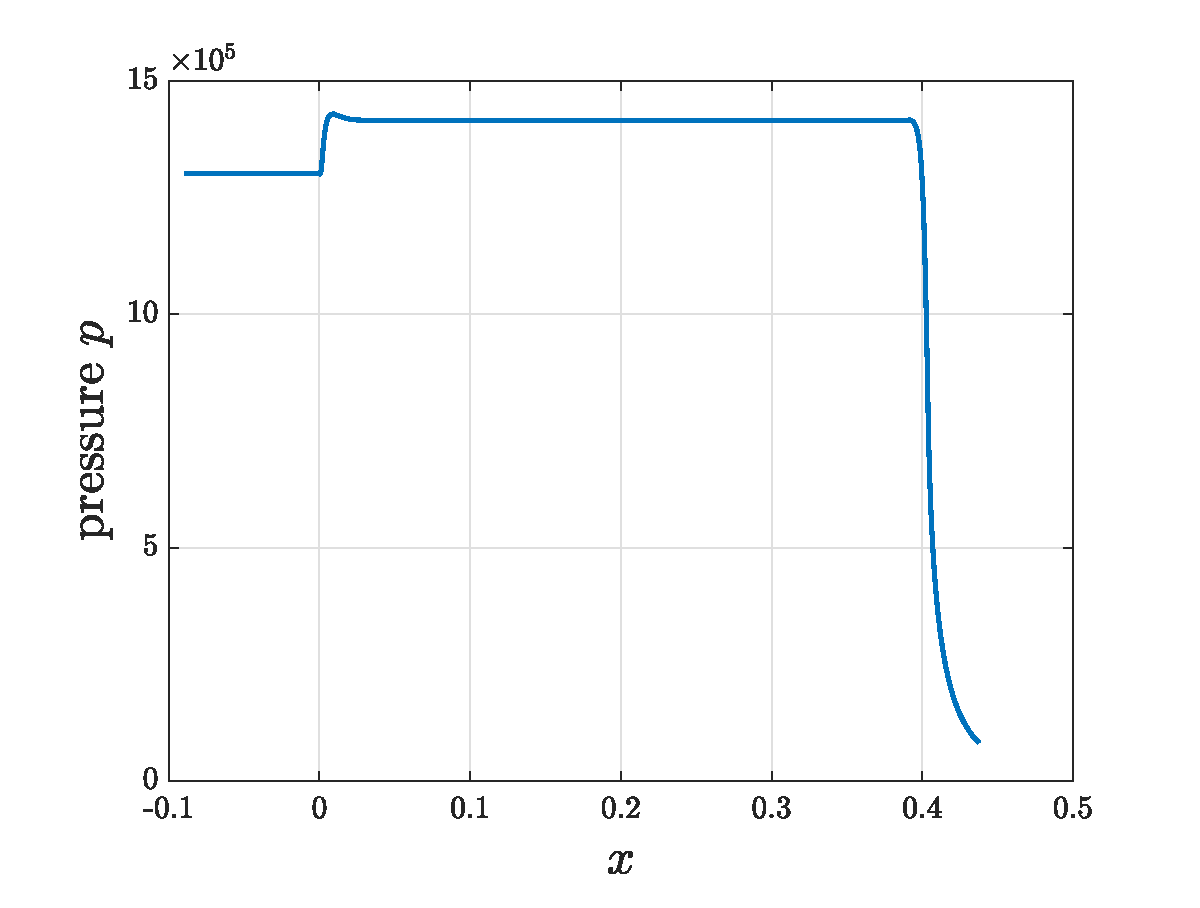
\includegraphics[width=\textwidth]{./pic/init_pressure}
%	\caption{} \label{fig:5p2.2a}
%\end{subfigure}
%\begin{subfigure}[]{0.47\linewidth}
%	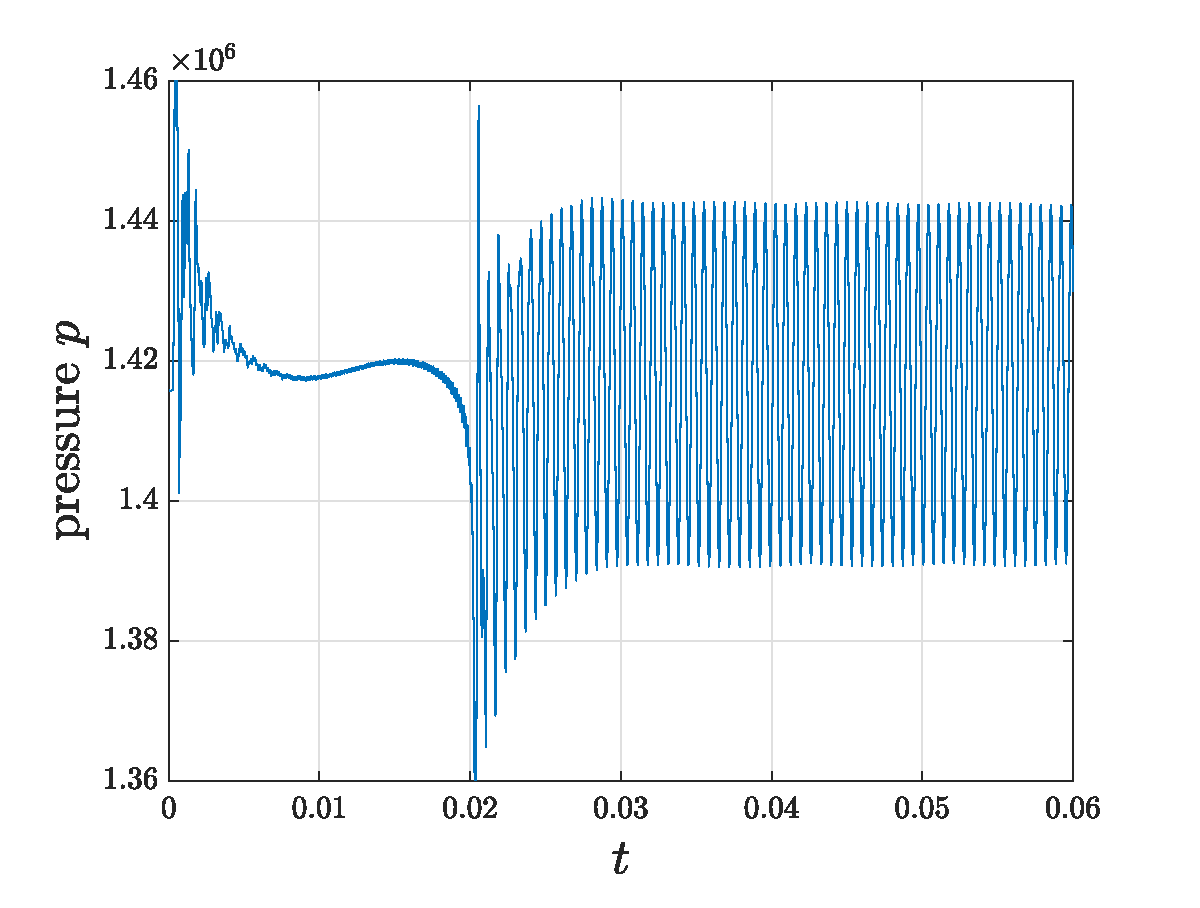
\includegraphics[width=\textwidth]{./pic/init_osc}
%	\caption{} \label{fig:5p2.2b}
%\end{subfigure} \\
%\begin{subfigure}[]{0.47\linewidth}
%	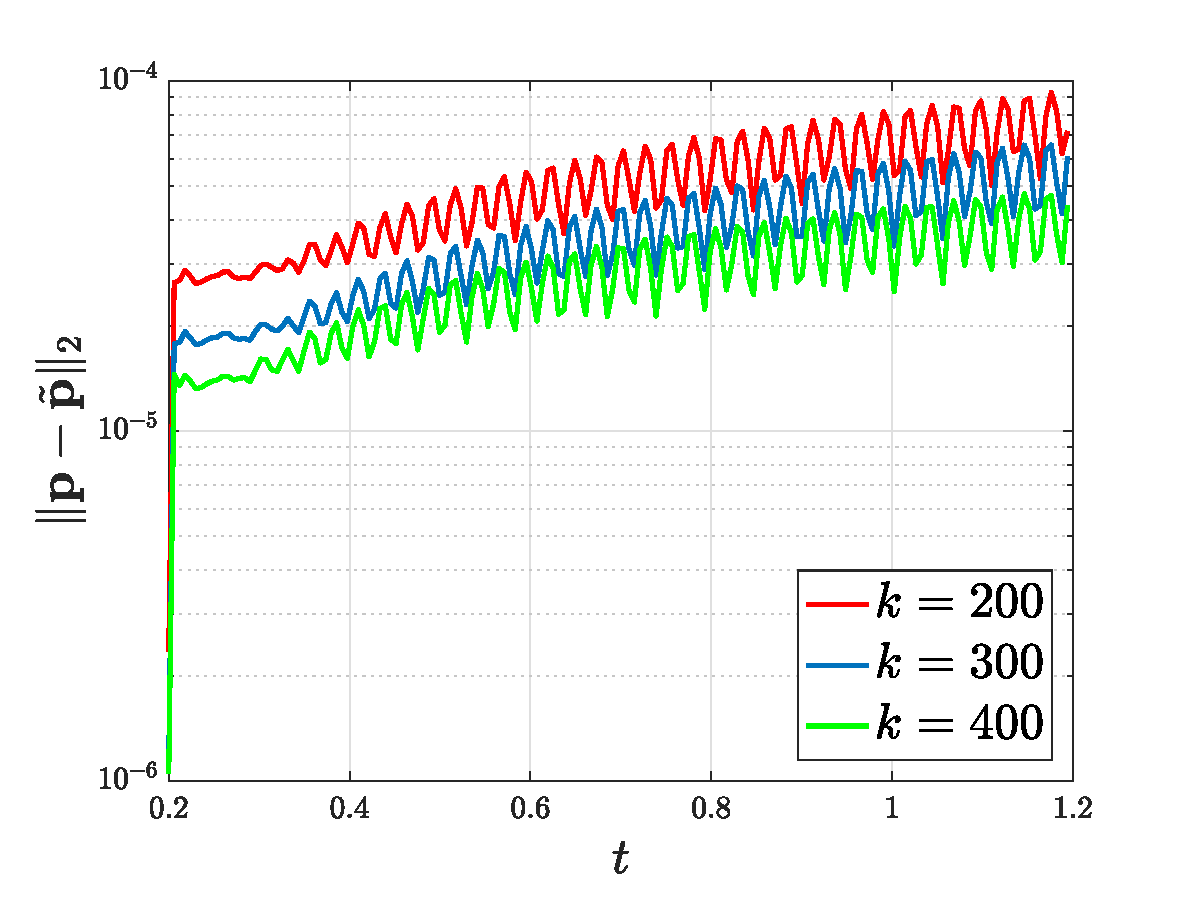
\includegraphics[width=\textwidth]{./pic/p_error}
%	\caption{} \label{fig:5p2.2c}
%\end{subfigure}
%\begin{subfigure}[]{0.47\linewidth}
%	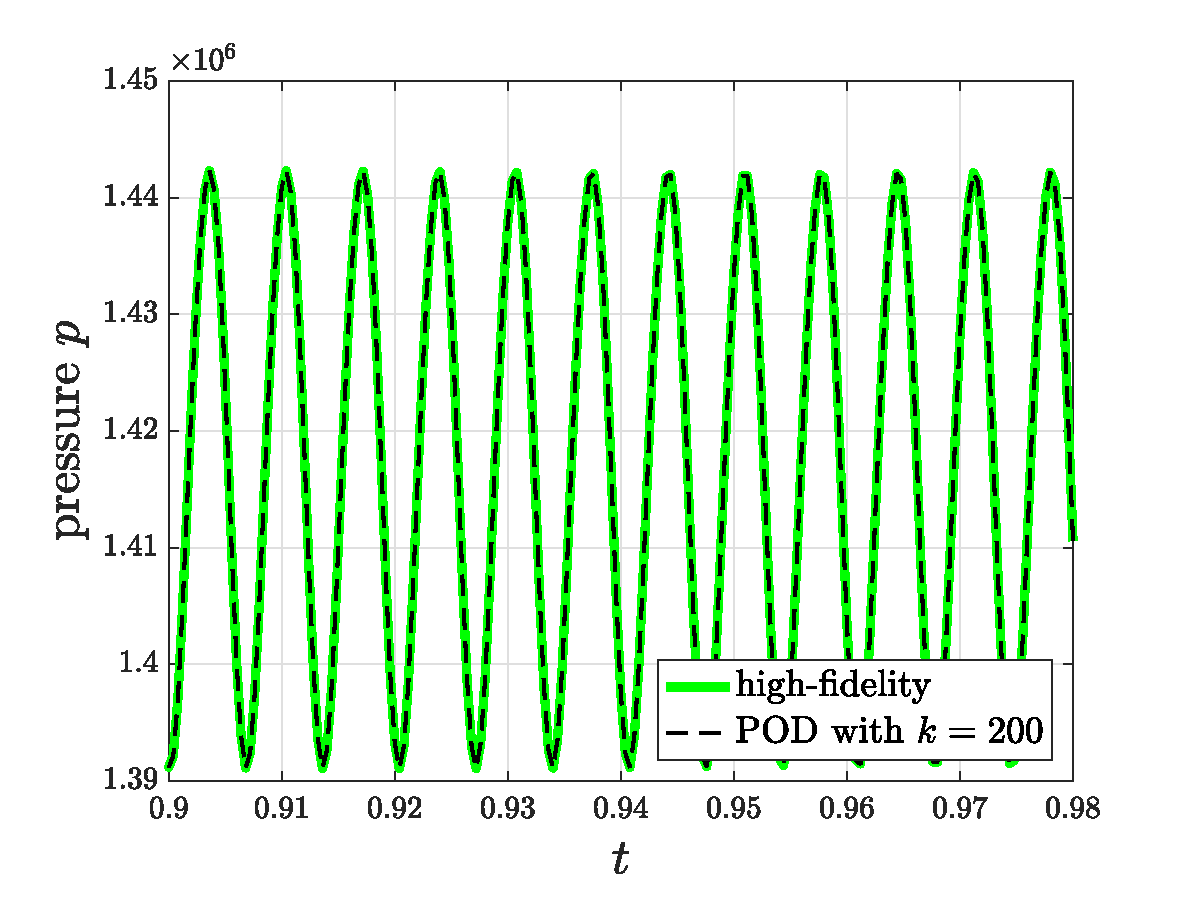
\includegraphics[width=\textwidth]{./pic/rom_freq}
%	\caption{} \label{fig:5p2.2d}
%\end{subfigure}
%\caption{(a) Pressure profile of the steady state. (b) Oscillatory mode of pressure located at $x=0.36$ for the unsteady flow. (c) Relative error between the high-fidelity and approximated pressure. (d) Approximation of the oscillations. }
%\label{fig:5p2.2}
%\end{figure}

%%%%%%%%%%%%%%%%%%%%%%%%%%%%%%%%%%%%%%%%%%%%
%%%%%%%%%%%%%%%%%%% Combustor %%%%%%%%%%%%%%%%%%%
%%%%%%%%%%%%%%%%%%%%%%%%%%%%%%%%%%%%%%%%%%%%
\begin{figure}
  \centering
  % Pressure steady
  \begin{subfigure}[]{0.48\linewidth}
          \includegraphics[scale=1]{Figures/paper-figure25.pdf}
%  \begin{tikzpicture}[scale=0.55]
%    \begin{axis}[ylabel = pressure $p$,
%                 xlabel=$x$,
%                 label style={font=\Large},
%                 legend pos=north east,
%                 %legend entries={$k=102$ Adv,$k=201$ Adv,$k=102$ Div,$k=201$ Div,$k=102$ Skew,$k=201$ Skew},
%                 legend style={font=\large},
%                 grid=both,
%                 ticks=both,
%                 width=1.4\linewidth, 
%                 height=1.0\linewidth,
%                 minor x tick num=1,
%                 minor y tick num=2,	
%                 %yticklabel style={/pgf/number format/.cd,fixed,precision=9},
%                 scaled x ticks = true,
%                 enlargelimits=false,
%                 scale only axis,
%%                 ymin=0,
%                 ymax = 1500000,
%                 samples = 100]
%                 \addplot[color=blue,style=solid,style=ultra thick]  table[x = x, y = pressure] {./data/Combustor/pressure_steady_state.txt};
%    \end{axis}%  
%  \end{tikzpicture}
  \caption{} \label{fig:5p2.2a}
  \label{steady_state}
  \end{subfigure}\hfill% 
  % Pressure oscilaltions
  \begin{subfigure}[]{0.48\linewidth}
        \includegraphics[scale=1]{Figures/paper-figure26.pdf}
%  \begin{tikzpicture}[scale=0.55]
%    \begin{axis}[ylabel = pressure $p$,
%                 xlabel=$t$,
%                 label style={font=\Large},
%                 legend pos=north east,
%                 %legend entries={$k=102$ Adv,$k=201$ Adv,$k=102$ Div,$k=201$ Div,$k=102$ Skew,$k=201$ Skew},
%                 legend style={font=\large},
%                 grid=both,
%                 ticks=both,
%                 width=1.4\linewidth, 
%                 height=1.0\linewidth,
%                 minor x tick num=1,
%                 minor y tick num=2,	
%                 %yticklabel style={/pgf/number format/.cd,fixed,precision=9},
%                 scaled x ticks = true,
%                 scaled y ticks = true,
%                 enlargelimits=false,
%                 scale only axis,
%                 ymin=0,
%%                 samples = 100,
%                 xmax = 0.06,
%                 ymin = 1360000,
%                 ymax = 1460000,
%                 tick label style={/pgf/number format/fixed} ]
%                 \addplot[color=blue,style=solid,style=thick]  table[x = t, y = pressure] {./data/Combustor/ciao.txt};
%    \end{axis}%  
%  \end{tikzpicture}
  \caption{} \label{fig:5p2.2b}
  \label{oscill_pressure}
  \end{subfigure}
  
% Total momentum
  \begin{subfigure}[]{0.48\linewidth}
      \includegraphics[scale=1]{Figures/paper-figure27.pdf}
%  \begin{tikzpicture}[scale=0.55]
%    \begin{semilogyaxis}[ylabel = $\| p-\tilde{p}\|_2$,
%                 xlabel=$t$,
%                 label style={font=\Large},
%                 legend pos=south east,
%                 legend entries={$k=200$,$k=300$,$k=300$},
%                 legend style={font=\large},
%                 grid=both,
%                 ticks=both,
%                 width=1.4\linewidth, 
%                 height=1.0\linewidth,
%                 minor x tick num=1,
%                 minor y tick num=2,	
%                 %yticklabel style={/pgf/number format/.cd,fixed,precision=9},
%                 scaled x ticks = true,
%                 scaled y ticks = true,
%                 enlargelimits=false,
%                 scale only axis,
%                 samples = 300,
%                 ymin = 0.000001,
%                 ymax = 0.0001]
%                 \addplot[color=red,style=solid,style=thick]  table[x = t, y = error] {./data/Combustor/error_200.txt};
%                 \addplot[color=blue,style=solid,style=thick]  table[x = t, y = error] {./data/Combustor/error_300.txt};
%                 \addplot[color=black!50!green,style=solid,style=thick]  table[x = t, y = error] {./data/Combustor/error_400.txt};
%    \end{semilogyaxis}%  
%  \end{tikzpicture}
  \caption{} \label{fig:5p2.2c}
  \label{error_growth_comb}
  \end{subfigure}\hfill% 
  % Pressure reduction  
  \begin{subfigure}[]{0.48\linewidth}
    \includegraphics[scale=1]{Figures/paper-figure28.pdf}
 % \begin{tikzpicture}[scale=0.55]
%    \begin{axis}[ylabel = pressure $p$,
%                 xlabel=$t$,
%                 label style={font=\Large},
%                 legend pos=north east,
%                 legend entries={High fidelity,  POD with $k=200$},
%                 legend style={font=\large},
%                 grid=both,
%                 ticks=both,
%                 width=1.4\linewidth, 
%                 height=1.0\linewidth,
%                 minor x tick num=1,
%                 minor y tick num=2,	
%                 %yticklabel style={/pgf/number format/.cd,fixed,precision=9},
%                 scaled x ticks = true,
%                 enlargelimits=false,
%                 scale only axis,
%                 xmin = 0.9,
%                 xmax = 0.98,
%                 ymin = 1390000,
%                 ymax = 1450000,
%                 tick label style={/pgf/number format/fixed} ]
%                 \addplot[color=green,style=solid,style=ultra thick]  table[x = t, y = pressure] {./data/Combustor/full.txt};
%                 \addplot[color=black,style=dashed,style=thick]  table[x = t, y = pressure] {./data/Combustor/red.txt};
%    \end{axis}%  
%  \end{tikzpicture}
  \caption{} \label{fig:5p2.2d}
  \label{oscill_focus}
  \end{subfigure}
  \caption{(\protect\subref{steady_state}) Pressure profile of the steady state.  (\protect\subref{oscill_pressure}) Oscillatory mode of pressure located at $x=0.36$ for the unsteady flow. (\protect\subref{error_growth_comb}) Relative error between the high-fidelity and approximated pressure. (\protect\subref{oscill_focus}) Approximation of the oscillations.} 
  \label{fig:5p2.2}
\end{figure}


The discontinuities that appear in the solution of \eqref{eq:5p2.10} suggests that a relatively large basis is required to resolve fine structures in the solution. Here, a POD basis is generated with $k=200$, $k=300$ and $k=400$ number of basis vectors. To avoid basis changes in the reduced system, only one POD basis is considered for $\rho$, $\rho u$ $\rho E$ and $\rho Y_{ox}$. The explicit SSP RK3 is then used to integrated the reduced system in time, for the unsteady system. The source terms are evaluated in the high-fidelity space and projected onto the reduced space. However, in principle, the DEIM can be applied to accelerate the evaluation this component. 

\Cref{fig:5p2.2c} shows the approximation error of the pressure, due to MOR. It is observed that the approximation is consistently improved as the number of basis vectors increases. Furthermore, the approximate solution maintains high accuracy over a relatively long time-integration. The oscillations of pressure is demonstrated in \Cref{fig:5p2.2d}. The overall behaviour of pressure is well approximated by the reduced system. Similar results are obtained for a POD basis with higher number of modes.

We note that the discrete form of \eqref{eq:5p2.10} is not in the full skew-symmetric form. Nonetheless, the quasi-skew-symmetric discretization offers remarkable stability preservation.

\section{Conclusions} \label{sec:con}

Conservation of nonlinear invariants are not, in general, guaranteed with conventional model reduction techniques. The violation of such invariants often result in a qualitatively wrong or unstable reduced system, even when the high-fidelity system is stable. This is particularly important for fluid flow, where conservation of the energy, as a nonlinear invariant of the system, is crucial for a correct numerical evaluation.

In this paper, we discuss that conservative properties of the skew-symmetric form for fluid flow can naturally be extended to the reduced system. Conventional MOR techniques preserves the skew-symmetry of differential operator which result in the conservation of quadratic invariants at the level of the reduced system. Furthermore, the reduced system also contains quadratic invariants with respect to the reduced variables that approximates the invariants of the high-fidelity system. This results in the construction of a physically meaningful reduced system, rather than a mere couple systems of differential equations.

Numerical experiments for the incompressible and compressible Euler equation confirms conservation of mass, momentum and energy for the reduced model with the skew-symmetric discretization. In contrast, when a non-skew-symmetric form, e.g. divergence form or advective form, is considered, MOR does not necessarily yield a stable reduced system. On the other hand the skew-symmetric form consistently yields a robust reduced system over long time-integration, even when the reduced space does not represent the high-fidelity solution accurately. 

Finally, a MOR of a quasi-skew-symmetric form for the CVRC model is presented. Although this model is not in a full skew-symmetric form and an explicit Runge-Kutta method used for time-integration, we still recover a reduced model with excellent stability properties. 

\section*{Acknowledgement} The work was partially supported by AFOSR under grant FA9550-17-1-9241 and by SNSF under the grant number P1ELP2-175039.


\bibliographystyle{plain}
\bibliography{references}

\end{document}
